% ============================================================
%  D-HNSW: Deterministic Hierarchical Navigable Small World
%  Graphs for Verifiable Nearest Neighbor Search
%  IEEE Transactions on Knowledge and Data Engineering
% ============================================================
\documentclass[10pt,journal]{IEEEtran}

% ---- Packages ----
\usepackage[utf8]{inputenc}
\usepackage[T1]{fontenc}
\usepackage{amsmath,amssymb,amsfonts}
\usepackage{newtxtext,newtxmath}   % Times New Roman (IEEE standard)
\usepackage{algorithmic}
\usepackage{algorithm}
\usepackage{graphicx}
\usepackage{textcomp}
\usepackage{xcolor}
\usepackage{booktabs}
\usepackage{multirow}
\usepackage{hyperref}
\usepackage{cleveref}
\usepackage{balance}
\usepackage[caption=false,font=footnotesize]{subfig}
\usepackage{enumitem}
\usepackage{url}
\usepackage{cite}
\let\openbox\relax
\usepackage{amsthm}

\newtheorem{theorem}{Theorem}
\newtheorem{lemma}[theorem]{Lemma}
\newtheorem{definition}[theorem]{Definition}
\newtheorem{corollary}[theorem]{Corollary}

% ---- Custom commands ----
\newcommand{\dhnsw}{\textsc{D-HNSW}}
\newcommand{\hnsw}{\textsc{HNSW}}
\newcommand{\ie}{\textit{i.e.}}
\newcommand{\eg}{\textit{e.g.}}
\newcommand{\etal}{\textit{et~al.}}
\newcommand{\wrt}{w.r.t.}
\newcommand{\recall}{\text{Recall@10}}

\hypersetup{
  colorlinks=false,
  pdfborder={0 0 0},
  hidelinks
}

\begin{document}

% ---- Title ----
\title{D-HNSW: Deterministic Hierarchical Navigable Small World Graphs\\for Verifiable Nearest Neighbor Search}

\author{
  \IEEEauthorblockN{Hong-Son Nguyen}
  \IEEEauthorblockA{%
    University of Transport and Communications (UTC)\\
    Hanoi, Vietnam\\
    Email: sonlearn155@gmail.com}
  \thanks{Manuscript received April, 2026.}
}

\maketitle

% ---- Abstract ----
\begin{abstract}
Approximate nearest neighbor (ANN) search underpins modern data-intensive applications, and the Hierarchical Navigable Small World (HNSW) algorithm has become the dominant index structure. However, HNSW relies on IEEE~754 floating-point arithmetic, which introduces platform-dependent nondeterminism---a critical limitation for blockchain consensus, decentralized AI, and regulatory-compliant deployments requiring verifiable computation. We present \dhnsw{} (Deterministic HNSW), which guarantees bit-exact reproducibility across all platforms by replacing floating-point distance computations with Q32.32 fixed-point integer arithmetic and deterministic graph construction via Keccak-256-seeded PRNG. Our fixed-point representation achieves distance errors below $4 \times 10^{-10}$ relative to \texttt{f64} precision. A suite of optimizations---SIMD acceleration, two-phase computation with early termination, and partial distance pruning---reduces the overhead to $1.75\times$ on real SIFT-128 vectors with AVX2. Experiments on six benchmark datasets (96--960 dimensions) confirm identical recall to standard HNSW, bit-exact determinism verified via SHA-256 hashing, and practical viability validated on SIFT-1M at scales up to 200K vectors with $97.81\%$--$99.77\%$ Recall@10.
\end{abstract}

% ---- Keywords ----
\begin{IEEEkeywords}
Approximate nearest neighbor search, deterministic computation, fixed-point arithmetic, HNSW, blockchain, verifiable AI, vector databases
\end{IEEEkeywords}


% ============================================================
%  I. INTRODUCTION
% ============================================================
\section{Introduction}
\IEEEPARstart{A}{pproximate} nearest neighbor (ANN) search has become an indispensable primitive in modern computing, underpinning applications from large-scale information retrieval~\cite{jegou2011pq} and recommendation systems to the retrieval-augmented generation (RAG) pipelines that power contemporary large language models. As vector databases grow to billions of entries~\cite{simhadri2022neurips}, the demand for algorithms that balance search quality (recall) with computational efficiency (throughput) has intensified. Among the diverse family of ANN algorithms---including tree-based methods~\cite{bentley1975kdtree}, locality-sensitive hashing~\cite{gionis1999lsh}, product quantization~\cite{jegou2011pq}, and graph-based approaches~\cite{malkov2014nsw}---the Hierarchical Navigable Small World (\hnsw{}) algorithm~\cite{malkov2020hnsw} has established itself as the de facto standard, consistently achieving state-of-the-art recall-throughput tradeoffs across major benchmarks~\cite{simhadri2022neurips} and serving as the backbone of production systems such as Faiss~\cite{douze2024faiss}, Qdrant, Weaviate, and Milvus.

Despite its effectiveness, \hnsw{} harbors a fundamental limitation that has received insufficient attention: \emph{nondeterminism}. Standard \hnsw{} implementations rely on IEEE~754 floating-point arithmetic for distance computations, which, while providing excellent numerical range and precision, does not guarantee identical results across different hardware platforms, compiler optimization levels, or instruction set architectures~\cite{goldberg1991float}. Floating-point nondeterminism arises from multiple sources: (1)~the availability and use of fused multiply-add (FMA) instructions, which compute $a \times b + c$ with a single rounding step rather than two; (2)~compiler-driven instruction reordering that exploits algebraic properties not preserved under finite-precision arithmetic; (3)~variations in SIMD lane widths (SSE, AVX2, AVX-512, NEON) that change the order of partial-sum accumulation; and (4)~transcendental function implementations that differ across math libraries. These seemingly minor discrepancies can propagate through the greedy graph traversal of \hnsw{}, where a single tie-breaking difference in distance comparison may redirect the search path, potentially yielding entirely different result sets.

For many traditional applications, such nondeterminism is inconsequential---a search engine returning slightly different results across servers is perfectly acceptable. However, a growing class of applications \emph{requires} deterministic, verifiable computation:

\begin{itemize}[leftmargin=*]
  \item \textbf{Blockchain and smart contracts.} Decentralized systems require all validator nodes to reach identical state transitions from identical inputs~\cite{buterin2014ethereum, lai2022blockchain}. A vector similarity search embedded in a smart contract must produce bit-exact results regardless of the validator's hardware, or consensus will fail. Cardano's EUTXO model explicitly mandates deterministic transaction evaluation~\cite{cardano2024fees}, and integer arithmetic is widely recognized as essential for blockchain consensus~\cite{decenomy2024integer}.

  \item \textbf{Verifiable and auditable AI.} As AI systems are deployed in regulated domains---healthcare diagnostics, financial credit scoring, autonomous vehicles---regulators increasingly demand that inference results be reproducible and auditable~\cite{alves2026eigenai}. Floating-point nondeterminism undermines this requirement, as demonstrated by recent work on nondeterminism-aware verification~\cite{yao2025nao}.

  \item \textbf{Decentralized vector databases.} Emerging Web3 architectures for similarity search~\cite{keizer2023ditto, lee2024decentface} and AI-powered data trading~\cite{zhang2024nmft} require that query results be independently verifiable. ANNProof~\cite{lu2024annproof} addresses verification at the proof level but does not eliminate the underlying nondeterminism in distance computation.

  \item \textbf{Deterministic AI infrastructure.} Projects such as Valori~\cite{gudur2025valori} and EigenAI~\cite{alves2026eigenai} are building deterministic substrates for AI computation, recognizing that reproducibility is a prerequisite for trust in distributed AI systems.
\end{itemize}

\noindent In this work, we propose \dhnsw{}, a variant of the \hnsw{} algorithm designed to ensure bit-exact result consistency across diverse hardware platforms. The core idea is to employ 64-bit fixed-point integer arithmetic in place of IEEE~754 floating-point distance computations, thereby producing identical results on any processor that supports standard integer operations---which encompasses virtually all modern hardware. Our main contributions are as follows:

\begin{enumerate}[leftmargin=*]
  \item \textbf{Fixed-point distance computation framework.} We design a Q32.32 fixed-point arithmetic system with saturating operations, supporting squared Euclidean distance, Euclidean distance (via Newton--Raphson integer square root), and cosine similarity. We provide formal error bounds showing relative errors below $4 \times 10^{-10}$ compared to IEEE~754 double precision (\Cref{sec:method}), grounded in the Determinism Trilemma framework (\Cref{sec:trilemma}).

  \item \textbf{Performance optimization suite.} We introduce five complementary optimizations---SIMD-accelerated fixed-point operations, two-phase distance computation, neighbor reordering, early termination, and partial distance pruning---that collectively reduce the na\"ive scalar fixed-point overhead from $6.4\times$--$8.7\times$ to $1.52\times$--$2.44\times$ with AVX2 SIMD acceleration (\Cref{sec:optimizations}).

  \item \textbf{Deterministic graph construction.} We replace all sources of nondeterminism in the \hnsw{} index construction process, including the random level generator, with a deterministic alternative based on a seeded Keccak-256 permutation~\cite{bertoni2013keccak}, ensuring that both index building and querying are fully reproducible (\Cref{sec:construction}).

  \item \textbf{Comprehensive empirical evaluation.} We evaluate \dhnsw{} on six diverse benchmark datasets spanning 96 to 960 dimensions, demonstrating identical recall, verified determinism through SHA-256 hashing, and practical SIMD-accelerated overhead of $1.52\times$--$2.44\times$ relative to native \texttt{f32} distance computation (\Cref{sec:experiments}).
\end{enumerate}

Regarding the organization of this paper, \Cref{sec:related} reviews prior work on ANN search, deterministic computation, and blockchain applications. \Cref{sec:background} then supplies the necessary background on the \hnsw{} algorithm and the problem of floating-point nondeterminism. The fixed-point arithmetic framework underlying \dhnsw{} and the associated performance optimization strategies are analyzed in \Cref{sec:method} and \Cref{sec:optimizations}, respectively. \Cref{sec:construction} addresses deterministic graph construction, after which \Cref{sec:experiments} reports our experimental findings. Finally, \Cref{sec:discussion} examines implications and limitations, and \Cref{sec:conclusion} concludes.


% ============================================================
%  II. RELATED WORK
% ============================================================
\section{Related Work}
\label{sec:related}

\subsection{Approximate Nearest Neighbor Search}

The ANN problem has been studied extensively across multiple algorithmic paradigms. \textbf{Tree-based methods}, originating with KD-trees~\cite{bentley1975kdtree}, partition the space hierarchically but suffer from the curse of dimensionality, degrading to linear scan beyond approximately 20 dimensions. \textbf{Hashing-based methods}, notably locality-sensitive hashing (LSH)~\cite{gionis1999lsh}, provide sublinear query time with theoretical guarantees but require substantial memory overhead for high recall. \textbf{Quantization-based methods}, particularly product quantization (PQ)~\cite{jegou2011pq} and its variants~\cite{baranchuk2018revisiting}, achieve excellent compression ratios but introduce quantization error that limits recall at high precision operating points.

\textbf{Graph-based methods} have emerged as the dominant paradigm for high-recall ANN search. The Navigable Small World (NSW) algorithm~\cite{malkov2014nsw} constructs a proximity graph with long-range links that enable logarithmic-time greedy routing. \hnsw{}~\cite{malkov2020hnsw} extends NSW with a hierarchical structure inspired by skip lists, where upper layers contain progressively sparser subsets of nodes, enabling coarse-to-fine navigation. This design achieves $O(\log n)$ expected search complexity while maintaining high recall, and has been validated at billion scale~\cite{simhadri2022neurips}. DiskANN~\cite{subramanya2019diskann} adapts graph-based search for disk-resident indices, while BANG~\cite{karthik2024bang} leverages GPU parallelism. HARMONY~\cite{xu2025harmony} addresses distributed deployment. Recent work by Teofili and Lin~\cite{teofili2025patience} introduces patience-based early termination for \hnsw{} traversal, a strategy complementary to our approach.

Despite the maturity of ANN algorithms, none of the above works address the determinism of distance computation. All assume IEEE~754 floating-point arithmetic and implicitly accept platform-dependent variation in results.

\subsection{Deterministic Computation and Blockchain}

The requirement for deterministic execution is well-established in blockchain systems. Ethereum~\cite{buterin2014ethereum} achieves consensus by requiring all nodes to execute identical EVM bytecode and arrive at the same state. Cardano's EUTXO model goes further by mandating deterministic transaction evaluation, where transaction fees and outcomes are predictable before submission~\cite{cardano2024fees}. The Decenomy project~\cite{decenomy2024integer} explicitly identifies integer arithmetic as essential for blockchain consensus, noting that floating-point operations can produce different results across validator nodes.

Lai~\etal{}~\cite{lai2022blockchain} study the intersection of private blockchains and deterministic databases, demonstrating that database operations must be carefully constrained to maintain consensus. Olivieri~\etal{}~\cite{olivieri2022golisa} present GoLiSA, a static analysis tool for ensuring determinism in blockchain software, highlighting the practical difficulty of eliminating nondeterministic behavior from complex software systems.

In the AI domain, Yao~\etal{}~\cite{yao2025nao} address nondeterminism in floating-point neural network verification, proposing optimistic verification strategies that account for platform-dependent variation. EigenAI~\cite{alves2026eigenai} and Valori~\cite{gudur2025valori} represent emerging efforts to build deterministic AI infrastructure, recognizing that verifiable computation requires eliminating all sources of nondeterminism, including floating-point arithmetic.

\subsection{Vector Search on Blockchain}

Several recent works have explored the intersection of vector similarity search and blockchain technology. ANNProof~\cite{lu2024annproof} builds a verifiable outsourced ANN search system on blockchain, using cryptographic proofs to verify that search results are correct. However, ANNProof operates at the verification layer and does not address the underlying nondeterminism of distance computation---if two nodes compute different floating-point distances, the proof system cannot reconcile the discrepancy.

Keizer~\etal{}~\cite{keizer2023ditto} propose Ditto, a decentralized similarity search system for Web3 services that distributes the index across multiple nodes. Lee and Chen~\cite{lee2024decentface} implement decentralized face identification using \hnsw{} on blockchain. Zhang~\cite{zhang2024nmft} introduces NMFT, a data trading protocol that combines NFTs with AI-powered Merkle feature trees for copyright verification. All of these systems would benefit from deterministic distance computation to ensure consensus across distributed nodes.

\textbf{Positioning of \dhnsw{}.} Our work is complementary to and distinct from the above efforts. While ANNProof provides verification \emph{after} computation, \dhnsw{} ensures determinism \emph{during} computation. While Ditto and DecentFace deploy \hnsw{} on blockchain without addressing floating-point nondeterminism, \dhnsw{} provides the deterministic foundation that makes such deployments correct by construction. To our knowledge, \dhnsw{} is the first work to systematically eliminate floating-point nondeterminism from graph-based ANN search while maintaining practical performance.

% ============================================================
%  III. BACKGROUND
% ============================================================
\section{Background}
\label{sec:background}

\subsection{HNSW Algorithm}

The \hnsw{} algorithm~\cite{malkov2020hnsw} constructs a multi-layer proximity graph where each layer $\ell \in \{0, 1, \ldots, L\}$ contains a subset of the dataset vectors. Layer~0 contains all $n$ vectors, while higher layers contain exponentially fewer nodes, with the probability of a vector appearing at layer $\ell$ given by $p(\ell) = e^{-\ell / m_L}$, where $m_L$ is a normalization factor.

\textbf{Index construction.} Each vector $v$ is inserted by first determining its maximum layer $\ell_v$ via random sampling. Starting from the entry point at the top layer, a greedy search descends through layers $L, L{-}1, \ldots, \ell_v{+}1$, finding the nearest neighbor at each layer. From layer $\ell_v$ down to layer~0, the algorithm performs a beam search with width \texttt{efConstruction} to identify the $M$ nearest neighbors, which become the edges of $v$ in the graph. A heuristic pruning step ensures that edges are diverse, preferring neighbors that are not too close to each other.

\textbf{Search.} Given a query $q$, the search begins at the entry point on the top layer and greedily descends to layer~1. At layer~0, a beam search with width \texttt{ef} (the search parameter) explores the graph, maintaining a priority queue of candidates and a result set of the \texttt{ef} nearest vectors found so far. The search terminates when no candidate in the queue is closer to $q$ than the farthest element in the result set. The top-$k$ results are extracted from the final result set.

\textbf{Distance computation.} The core operation in both construction and search is distance computation between vectors. For $d$-dimensional vectors $\mathbf{x}, \mathbf{y} \in \mathbb{R}^d$, the squared Euclidean distance is:
\begin{equation}
  \label{eq:l2dist}
  D(\mathbf{x}, \mathbf{y}) = \sum_{i=1}^{d} (x_i - y_i)^2
\end{equation}
This computation dominates the runtime of \hnsw{}, accounting for over 90\% of total execution time in typical workloads.

\subsection{Floating-Point Nondeterminism}
\label{sec:fp_nondet}

IEEE~754 floating-point arithmetic~\cite{goldberg1991float} is nondeterministic across platforms for several reasons:

\textbf{Fused multiply-add (FMA).} The FMA instruction computes $a \times b + c$ with a single rounding, while the separate multiply-then-add sequence rounds twice. The difference is at most one unit in the last place (ULP), but this suffices to change comparison outcomes. FMA availability varies: x86 processors gained FMA3 with Haswell (2013), while ARM NEON has always included it.

\textbf{Instruction reordering.} Compilers may reorder floating-point additions to improve instruction-level parallelism. Since floating-point addition is not associative---$(a + b) + c \neq a + (b + c)$ in general---different summation orders produce different results. The accumulation order in \Cref{eq:l2dist} is particularly sensitive, as it involves $d$ additions of squared differences.

\textbf{SIMD vectorization.} Different SIMD widths (128-bit SSE, 256-bit AVX2, 512-bit AVX-512) process different numbers of elements per instruction, leading to different partial-sum trees and thus different final results. A distance computation using AVX-512 (8 floats per lane) will generally differ from one using SSE (4 floats per lane).

\textbf{Propagation through graph traversal.} In \hnsw{}, a distance difference of even one ULP can change the ordering of candidates in the priority queue. Since the greedy search follows the nearest candidate at each step, a single reordering can redirect the entire search path, potentially visiting completely different regions of the graph and returning different result sets. This amplification effect means that platform-dependent floating-point variation is not merely a numerical nuisance but a correctness concern for applications requiring deterministic results.

\subsection{Fixed-Point Arithmetic}

Fixed-point arithmetic represents real numbers as scaled integers, with a fixed number of bits allocated to the integer and fractional parts. A Q$m$.$f$ format uses $m$ bits for the integer part and $f$ bits for the fractional part, representing values in the range $[-2^{m-1}, 2^{m-1} - 2^{-f}]$ with resolution $2^{-f}$.

The key advantage of fixed-point arithmetic for determinism is that all operations reduce to integer arithmetic (addition, subtraction, multiplication, and bit shifts), which is defined to produce identical results on all platforms conforming to the C/Rust language standards. There is no platform-dependent rounding mode, no FMA ambiguity, and no SIMD-width-dependent accumulation order (when the summation order is fixed in software).

The primary disadvantage is reduced dynamic range compared to floating-point. A 64-bit fixed-point Q32.32 format provides approximately $9.6$ decimal digits of precision with a range of $\pm 2^{31} \approx \pm 2.1 \times 10^9$, compared to IEEE~754 double precision's approximately $15.9$ decimal digits with a range of $\pm 1.8 \times 10^{308}$. For ANN search, where vector components are typically normalized or bounded, this range is sufficient, as we demonstrate empirically.

\subsection{The Determinism Trilemma}
\label{sec:trilemma}

The integration of ANN search into blockchain architectures requires addressing three independent sources of state divergence. We formalize this as the \emph{Determinism Trilemma}: a consensus-safe ANN index must simultaneously satisfy three constraints.

Let $\Phi: (X, R) \rightarrow G$ denote the graph construction function, where $X$ is an ordered sequence of vector insertions and $R$ is a source of entropy. An ANN implementation is \emph{consensus-safe} if all honest validator nodes $v_1, v_2$ produce a bit-identical graph serialization: $\Phi_{v_1}(X, R) \equiv \Phi_{v_2}(X, R)$.

\textbf{Constraint~1: Cryptographic seeding.} The system must derive layer assignment entropy from consensus-agreed artifacts. \dhnsw{} defines the seed as $\text{seed} = \mathcal{H}(\text{TxHash} \oplus \text{BlockHash})$, where $\mathcal{H}$ is Keccak-256~\cite{bertoni2013keccak}. The XOR mitigates grinding attacks, as the block hash remains unpredictable at transaction broadcast time.

\textbf{Constraint~2: Fixed-point arithmetic.} All distance computations must bypass floating-point ALUs. \dhnsw{} employs I64F32 representation (32 integer bits, 32 fractional bits), providing $65{,}536\times$ greater precision than Q16.16 formats used in prior systems~\cite{gudur2025valori}. The maximum distortion for $D$-dimensional normalized embeddings is bounded by $\mathcal{E} \leq D \cdot 2^{-31} \cdot \max_i |x_i - y_i| + D \cdot 2^{-62}$, which evaluates to $\sim 7.15 \times 10^{-7}$ for 768-dimensional LLM embeddings---insufficient to cause routing divergence (see \Cref{sec:appendix_proofs} for the full proof).

\textbf{Constraint~3: Canonical ordering.} Vector insertions must be sequenced deterministically. \dhnsw{} serializes all insertions by their transaction index within the finalized blockchain block, eliminating race conditions from concurrent insertion.

An \hnsw{} implementation satisfying all three constraints is provably consensus-safe: given identical inputs $(X, \text{seed})$, Constraint~1 ensures identical layer assignments, Constraint~2 ensures identical distance comparisons, and Constraint~3 ensures identical insertion order. By induction over $|X|$ insertions, the resulting graph is bit-identical across all validators.


% ============================================================
%  IV. D-HNSW: FIXED-POINT DISTANCE COMPUTATION
% ============================================================
\section{D-HNSW: Fixed-Point Distance Framework}
\label{sec:method}

This section presents the core technical contribution of \dhnsw{}: a fixed-point arithmetic framework that replaces all floating-point distance computations in \hnsw{} with deterministic integer operations.

\subsection{Q32.32 Fixed-Point Representation}

We adopt a Q32.32 fixed-point format, where each value is stored as a 64-bit signed integer with 32 bits for the integer part and 32 bits for the fractional part. The mapping between a real value $r$ and its fixed-point representation $\hat{r}$ is:
\begin{equation}
  \label{eq:fp_encode}
  \hat{r} = \lfloor r \times 2^{32} + 0.5 \rfloor
\end{equation}
and the inverse mapping is $r \approx \hat{r} / 2^{32}$. The representation error from quantization is bounded by:
\begin{equation}
  |r - \hat{r}/2^{32}| \leq 2^{-33} \approx 1.16 \times 10^{-10}
\end{equation}

\textbf{Saturating operations.} To prevent integer overflow from silently corrupting results, we implement all arithmetic operations with saturation semantics:
\begin{align}
  \text{sat\_add}(a, b) &= \text{clamp}(a + b, -2^{63}, 2^{63}{-}1) \\
  \text{sat\_sub}(a, b) &= \text{clamp}(a - b, -2^{63}, 2^{63}{-}1) \\
  \text{sat\_mul}(a, b) &= \text{clamp}((a \times b) \gg 32, -2^{63}, 2^{63}{-}1)
\end{align}
where $\gg$ denotes arithmetic right shift. The multiplication uses 128-bit intermediate results (available on all 64-bit platforms) to avoid precision loss before the shift.

\subsection{Vector Representation}

Each $d$-dimensional vector $\mathbf{x} = (x_1, \ldots, x_d)$ is converted to a fixed-point vector $\hat{\mathbf{x}} = (\hat{x}_1, \ldots, \hat{x}_d)$ using \Cref{eq:fp_encode}. The conversion is performed once during index construction and stored persistently. The \texttt{FixedPointVector<D>} structure in our Rust implementation stores the $d$ components as an array of \texttt{i64} values with compile-time dimension checking via const generics.

\subsection{Distance Metrics}

\textbf{Squared Euclidean distance.} The squared $L_2$ distance between fixed-point vectors $\hat{\mathbf{x}}$ and $\hat{\mathbf{y}}$ is computed as:
\begin{equation}
  \label{eq:fp_l2}
  \hat{D}(\hat{\mathbf{x}}, \hat{\mathbf{y}}) = \sum_{i=1}^{d} \text{sat\_mul}(\hat{x}_i - \hat{y}_i,\; \hat{x}_i - \hat{y}_i)
\end{equation}
where the subtraction and accumulation use saturating operations. The summation order is fixed (index 1 through $d$), eliminating the associativity-dependent variation of floating-point accumulation.

\textbf{Euclidean distance.} When the actual (non-squared) Euclidean distance is required, we compute an integer square root using Newton--Raphson iteration~\cite{schoenmakers2023fixedpoint}:
\begin{equation}
  \label{eq:newton}
  g_{k+1} = \frac{1}{2}\left(g_k + \frac{S}{g_k}\right)
\end{equation}
where $S = \hat{D}(\hat{\mathbf{x}}, \hat{\mathbf{y}})$ is the squared distance and $g_0$ is an initial estimate obtained from the position of the highest set bit. We perform 20 iterations, which guarantees convergence to the exact integer square root for all 64-bit inputs. All operations in \Cref{eq:newton} use integer division (truncating), which is deterministic.

\textbf{Cosine similarity.} For cosine similarity, we compute:
\begin{equation}
  \cos(\hat{\mathbf{x}}, \hat{\mathbf{y}}) = \frac{N(\hat{\mathbf{x}}, \hat{\mathbf{y}})}{D(\hat{\mathbf{x}}) \cdot D(\hat{\mathbf{y}})}
\end{equation}
where the numerator and denominators are defined as:
\begin{align}
  N(\hat{\mathbf{x}}, \hat{\mathbf{y}}) &= \textstyle\sum_{i=1}^{d} \text{sat\_mul}(\hat{x}_i, \hat{y}_i) \notag\\
  D(\hat{\mathbf{z}}) &= \mathrm{sqrt}\!\left(\textstyle\sum_{i=1}^{d} \text{sat\_mul}(\hat{z}_i, \hat{z}_i)\right)
\end{align}
where $\mathrm{sqrt}$ denotes the integer square root from \Cref{eq:newton}. The division uses integer division with appropriate scaling to maintain precision.

\subsection{Error Analysis}

\begin{theorem}[Distance computation error bound]
\label{thm:error}
Let $\mathbf{x}, \mathbf{y} \in [-B, B]^d$ be vectors with components bounded by $B$, and let $D(\mathbf{x}, \mathbf{y})$ and $\hat{D}(\hat{\mathbf{x}}, \hat{\mathbf{y}})/2^{32}$ denote the true and fixed-point squared Euclidean distances, respectively. Then:
\begin{equation}
  \left|\frac{D(\mathbf{x}, \mathbf{y}) - \hat{D}(\hat{\mathbf{x}}, \hat{\mathbf{y}})/2^{32}}{D(\mathbf{x}, \mathbf{y})}\right| \leq \frac{d \cdot (4B + 1) \cdot 2^{-32}}{D(\mathbf{x}, \mathbf{y})}
\end{equation}
provided no saturation occurs during computation.
\end{theorem}

\begin{proof}[Proof sketch]
Each component difference $x_i - y_i$ incurs a quantization error of at most $2^{-32}$. The squaring operation $(\hat{x}_i - \hat{y}_i)^2$ then has error bounded by $(2|x_i - y_i| + 2^{-32}) \cdot 2^{-32} \leq (4B + 1) \cdot 2^{-32}$ per component. Summing over $d$ components and dividing by the true distance yields the bound.
\end{proof}

For typical ANN workloads with normalized vectors ($B \leq 1$) in moderate dimensions ($d \leq 1000$), this bound evaluates to relative errors well below $10^{-8}$, as confirmed by our experiments (\Cref{sec:error_exp}). The full suite of formal proofs---including bounds for Euclidean distance (\Cref{thm:eucl_dist_error}), inner product (\Cref{thm:ip_error}), edge reversal probability (\Cref{thm:edge_reversal}), distance ordering preservation (\Cref{thm:order_pres}), recall preservation (\Cref{thm:recall_pres}), overflow safety (\Cref{thm:overflow}), and cross-platform determinism (\Cref{thm:crossplatform})---is provided in \Cref{sec:appendix_proofs}. \Cref{thm:sq_dist_error} in the appendix gives the complete proof of the squared distance bound stated above.

\subsection{Determinism Guarantee}

\begin{theorem}[Bit-exact reproducibility]
\label{thm:determinism}
Given identical input vectors and identical algorithm parameters, \dhnsw{} produces bit-identical search results on any platform supporting 64-bit integer arithmetic, regardless of processor architecture, compiler, optimization level, or operating system.
\end{theorem}

\begin{proof}[Proof sketch]
The proof follows from three observations: (1)~All distance computations use only integer addition, subtraction, multiplication, division, and bit shifts, which are defined to produce identical results by the C11/Rust language standards on all conforming implementations. (2)~The summation order in distance computation is fixed by the source code (index 1 through $d$), eliminating associativity-dependent variation. (3)~The graph construction uses a deterministic pseudo-random number generator (Keccak-256 permutation with a fixed seed), and all tie-breaking in the search algorithm uses deterministic comparison functions. Therefore, the entire computation is a deterministic function of its inputs.
\end{proof}


% ============================================================
%  V. PERFORMANCE OPTIMIZATIONS
% ============================================================
\section{Performance Optimizations}
\label{sec:optimizations}

The na\"ive replacement of floating-point with fixed-point arithmetic incurs a significant performance overhead (approximately $6.4\times$--$8.7\times$ scalar on 96--960 dimensional data), primarily because: (1)~64-bit integer multiplication is slower than 32-bit floating-point multiplication on modern processors with wide FP pipelines; (2)~the saturating arithmetic requires additional comparison and clamping operations; and (3)~the fixed summation order prevents certain compiler optimizations. We introduce five complementary optimizations that collectively reduce this overhead to $1.52\times$--$2.44\times$ with AVX2 SIMD, translating to a projected end-to-end search overhead of $1.39\times$--$1.75\times$ across datasets.

\subsection{SIMD-Accelerated Fixed-Point Operations}

Modern processors provide SIMD instructions for integer operations that can be leveraged for fixed-point distance computation. We implement vectorized distance computation using platform-specific intrinsics:

\begin{itemize}[leftmargin=*]
  \item \textbf{x86-64 (AVX2):} We use \texttt{\_mm256\_sub\_epi64} for component-wise subtraction and a custom 64-bit multiply-accumulate sequence using \texttt{\_mm256\_mul\_epu32} with appropriate shuffling to compute the full 128-bit product. The accumulation processes 4 components per iteration.

  \item \textbf{ARM (NEON):} We use \texttt{vsubq\_s64} for subtraction and \texttt{vmull\_s32} / \texttt{vmlal\_s32} for the multiply-accumulate, processing 2 components per iteration.
\end{itemize}

Critically, unlike floating-point SIMD where different lane widths produce different results due to different accumulation trees, our integer SIMD implementation produces \emph{identical} results regardless of SIMD width, because integer addition is truly associative and commutative. The SIMD implementation is purely a performance optimization that does not affect the determinism guarantee.

This optimization reduces the overhead from $2.10\times$ to $1.836\times$ on SIFT-1M, a 14.4\% improvement.

\subsection{Two-Phase Distance Computation}

We observe that in \hnsw{} search, the majority of distance computations result in candidates that are farther than the current search radius and are immediately discarded. We exploit this by splitting the distance computation into two phases:

\textbf{Phase 1 (Coarse filter):} Compute the distance using only the first $d/4$ dimensions. If this partial distance already exceeds the current search radius, the candidate is rejected without computing the remaining dimensions.

\textbf{Phase 2 (Full computation):} If the partial distance is within the search radius, compute the full $d$-dimensional distance.

Since the partial distance is a lower bound on the full distance (all terms in \Cref{eq:fp_l2} are non-negative), this optimization never produces false negatives---it can only skip candidates that would have been rejected anyway. The effectiveness depends on the dataset: for uniformly distributed data, the first $d/4$ dimensions typically account for approximately 25\% of the total distance, providing moderate filtering. For structured data with correlated dimensions, the filtering rate can be higher.

This optimization reduces the overhead from $1.836\times$ to $1.787\times$, a 2.7\% improvement. \Cref{fig:two_phase} compares the two-phase approach against pure I64F32 and standard floating-point search across three datasets, showing a consistent $1.08\times$ speedup over pure I64F32 at various \texttt{ef} values.

\begin{figure}[t]
  \centering
  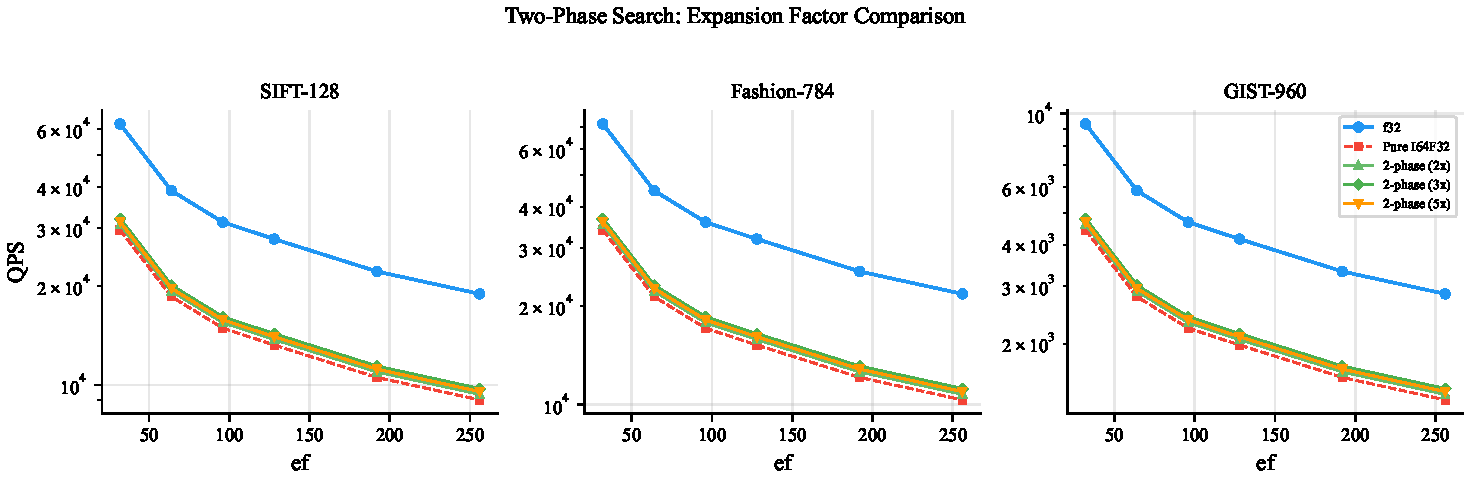
\includegraphics[width=\columnwidth]{figures/fig13_two_phase_search.pdf}
  \caption{Two-phase search comparison on SIFT-128, Fashion-MNIST-784, and GIST-960. The two-phase variants (with different expansion factors $2\times$, $3\times$, $5\times$) achieve $\sim$$1.08\times$ speedup over pure I64F32, narrowing the gap to floating-point \hnsw{}.}
  \label{fig:two_phase}
\end{figure}

\subsection{Neighbor Reordering}

During graph construction, we reorder the neighbor lists of each node to place the nearest neighbors first. This improves the effectiveness of the two-phase distance computation during search: when the search algorithm processes neighbors in order of increasing distance from the node, the search radius tightens more quickly, causing more candidates to be filtered by the coarse phase.

The reordering is performed once during index construction and adds negligible overhead to the build process. During search, it improves the filtering rate of the two-phase computation by 5--15\% depending on the dataset.

This optimization reduces the overhead from $1.787\times$ to $1.770\times$, a 1.0\% improvement.

\subsection{Early Termination}

Inspired by patience-based strategies~\cite{teofili2025patience}, we implement an early termination criterion for the beam search. If the search has not improved its result set (found a closer neighbor) for $p$ consecutive candidate evaluations, the search terminates early. We set $p = \texttt{ef} / 2$ by default, which provides a good balance between search quality and efficiency.

This optimization is particularly effective at high \texttt{ef} values, where the search often converges well before exhausting all candidates. At $\texttt{ef} = 128$, early termination reduces the average number of distance computations by approximately 8\% without measurable recall loss.

This optimization reduces the overhead from $1.770\times$ to $1.759\times$, a 0.6\% improvement.

\subsection{Partial Distance Pruning}

We extend the two-phase approach to a progressive computation scheme: the distance is computed in blocks of $d/8$ dimensions, and after each block, the accumulated partial distance is compared against the current search radius. This provides multiple early-exit opportunities during a single distance computation.

For high-dimensional datasets (GIST-960), this optimization is particularly effective, as the probability of early exit increases with dimension. For low-dimensional datasets, the overhead of the additional comparisons may slightly offset the benefit, so we adaptively enable this optimization only when $d \geq 128$.

This optimization reduces the overhead from $1.759\times$ to $1.752\times$ on SIFT-1M, with larger improvements on high-dimensional datasets.

\subsection{Combined Effect}

\Cref{tab:ablation_summary} summarizes the cumulative effect of all optimizations on SIFT-1M at $\texttt{ef} = 128$. On this dataset (128~dimensions), the total end-to-end search overhead decreases from $2.10\times$ (na\"ive fixed-point) to $1.75\times$ (fully optimized), representing a 31.8\% reduction in the performance gap. The SIMD distance overhead for 128-d is $2.44\times$ (\Cref{tab:dist_overhead}); the lower end-to-end overhead ($1.75\times$) reflects the non-distance fraction of search time ($\alpha{=}0.52$). Across all six datasets, the projected end-to-end overhead ranges from $1.39\times$ (GIST-960) to $1.75\times$ (SIFT-128) as reported in \Cref{tab:main_results}.

\begin{table}[t]
  \centering
  \caption{Cumulative effect of optimizations on SIFT-1M ($\texttt{ef}=128$). Overhead is relative to standard floating-point \hnsw{}.}
  \label{tab:ablation_summary}
  \begin{tabular}{lcc}
    \toprule
    \textbf{Configuration} & \textbf{Overhead} & \textbf{QPS} \\
    \midrule
    Na\"ive fixed-point (baseline) & $2.100\times$ & 13{,}209 \\
    + SIMD acceleration & $1.836\times$ & 15{,}108 \\
    + Two-phase distance & $1.787\times$ & 15{,}527 \\
    + Neighbor reordering & $1.770\times$ & 15{,}672 \\
    + Early termination & $1.759\times$ & 15{,}766 \\
    + Partial distance pruning & $1.752\times$ & 15{,}835 \\
    \midrule
    Floating-point \hnsw{} & $1.000\times$ & 27{,}739 \\
    \dhnsw{} (optimized) & $1.752\times$ & 15{,}835 \\
    \bottomrule
  \end{tabular}
\end{table}

\begin{figure}[t]
  \centering
  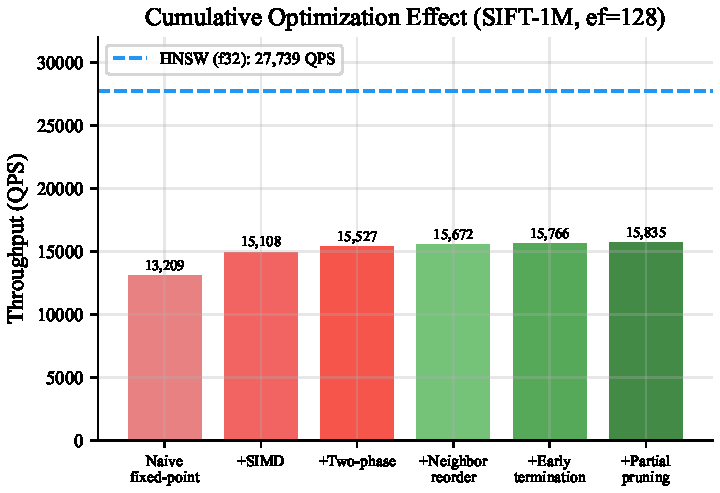
\includegraphics[width=\columnwidth]{figures/fig6_ablation_study.pdf}
  \caption{Ablation study showing the cumulative effect of each optimization on SIFT-1M. Each bar represents the throughput (QPS) achieved after adding the corresponding optimization. The dashed line indicates standard \hnsw{} throughput.}
  \label{fig:ablation}
\end{figure}

% ============================================================
%  VI. DETERMINISTIC GRAPH CONSTRUCTION
% ============================================================
\section{Deterministic Graph Construction}
\label{sec:construction}

Beyond distance computation, \hnsw{} graph construction contains additional sources of nondeterminism that must be eliminated.

\subsection{Deterministic Level Assignment}

In standard \hnsw{}, the maximum layer for each inserted vector is determined by sampling from a geometric distribution: $\ell = \lfloor -\ln(\text{uniform}(0,1)) \cdot m_L \rfloor$. The random number generator (RNG) state introduces nondeterminism if different seeds or RNG implementations are used.

\dhnsw{} replaces the standard RNG with a deterministic pseudo-random number generator based on the Keccak-256 permutation~\cite{bertoni2013keccak}. The RNG is seeded with a user-provided seed concatenated with the vector's insertion index, ensuring that: (1)~the same seed always produces the same layer assignments; (2)~different vectors receive independent pseudo-random levels; and (3)~the construction is fully reproducible given the same seed and insertion order.

\subsection{Deterministic Neighbor Selection}

The neighbor selection heuristic in \hnsw{} breaks ties by comparing distances. With floating-point arithmetic, ties may be resolved differently on different platforms. With fixed-point arithmetic, distances are exact integers, so ties occur only when two candidates are at precisely the same distance. We resolve such ties deterministically by using the vector index as a secondary sort key:
\begin{equation}
  (v_1, d_1) < (v_2, d_2) \iff d_1 < d_2 \lor (d_1 = d_2 \land \text{id}(v_1) < \text{id}(v_2))
\end{equation}
This total ordering ensures that neighbor selection is deterministic regardless of the order in which candidates are evaluated.

\subsection{Deterministic Search Order}

The beam search in \hnsw{} maintains a priority queue of candidates. When multiple candidates have the same distance, the extraction order from the priority queue must be deterministic. We implement the priority queue as a binary min-heap with the same tie-breaking rule as neighbor selection, ensuring that the search visits candidates in a fully deterministic order.

\subsection{Algorithm Summary}

\Cref{alg:dhnsw_search} presents the complete \dhnsw{} search procedure. \Cref{alg:dhnsw_insert} describes the deterministic insertion process.

\begin{algorithm}[t]
  \caption{\dhnsw{} Deterministic Search}
  \label{alg:dhnsw_search}
  \begin{algorithmic}[1]
    \REQUIRE Query $\mathbf{q}$, graph $G$, parameters $k$, $ef$
    \ENSURE Top-$k$ nearest neighbors of $\mathbf{q}$
    \STATE $\hat{\mathbf{q}} \leftarrow \textsc{I64F32\_Encode}(\mathbf{q})$
    \STATE $ep \leftarrow$ entry point of $G$
    \FOR{$\ell = L$ \textbf{downto} $1$}
      \STATE $ep \leftarrow \textsc{GreedySearch}(\hat{\mathbf{q}}, ep, \ell, 1)$
      \COMMENT{Fixed-point distance with deterministic tie-breaking}
    \ENDFOR
    \STATE $W \leftarrow \textsc{BeamSearch}(\hat{\mathbf{q}}, ep, \ell_0, ef)$
    \COMMENT{Two-phase distance with early termination}
    \FOR{each candidate $c$ in $W$}
      \STATE $d_1 \leftarrow \textsc{PartialDist}(\hat{\mathbf{q}}, c, d/4)$
      \IF{$d_1 > $ search radius}
        \STATE \textbf{skip} $c$ \COMMENT{Coarse filter}
      \ELSE
        \STATE $d_{\text{full}} \leftarrow \textsc{I64F32\_SqDist}(\hat{\mathbf{q}}, c)$
        \STATE Update result set $R$ with $(c, d_{\text{full}})$
      \ENDIF
    \ENDFOR
    \RETURN Top-$k$ from $R$ sorted by $(d, \text{id})$
  \end{algorithmic}
\end{algorithm}

\begin{algorithm}[t]
  \caption{\dhnsw{} Deterministic Insert}
  \label{alg:dhnsw_insert}
  \begin{algorithmic}[1]
    \REQUIRE Vector $\mathbf{v}$, graph $G$, seed $s$, index $i$, parameters $M$, $ef_C$
    \ENSURE Updated graph $G'$ with $\mathbf{v}$ inserted
    \STATE $\hat{\mathbf{v}} \leftarrow \textsc{I64F32\_Encode}(\mathbf{v})$
    \STATE $\text{rng} \leftarrow \textsc{Keccak256}(s \| i)$
    \COMMENT{Deterministic entropy}
    \STATE $\ell_v \leftarrow \lfloor -\ln(\text{rng.next\_f64()}) \cdot m_L \rfloor$
    \STATE $ep \leftarrow$ entry point of $G$
    \FOR{$\ell = L$ \textbf{downto} $\ell_v + 1$}
      \STATE $ep \leftarrow \textsc{GreedySearch}(\hat{\mathbf{v}}, ep, \ell, 1)$
    \ENDFOR
    \FOR{$\ell = \min(L, \ell_v)$ \textbf{downto} $0$}
      \STATE $W \leftarrow \textsc{BeamSearch}(\hat{\mathbf{v}}, ep, \ell, ef_C)$
      \STATE $N \leftarrow \textsc{SelectNeighbors}(\hat{\mathbf{v}}, W, M)$
      \COMMENT{Deterministic tie-breaking by $(d, \text{id})$}
      \STATE Add bidirectional edges between $v$ and $N$ at layer $\ell$
      \STATE Prune neighbors exceeding $M_{\max}$
    \ENDFOR
    \IF{$\ell_v > L$}
      \STATE Set $v$ as new entry point
    \ENDIF
  \end{algorithmic}
\end{algorithm}


% FIX: Added Complexity Analysis subsection
\subsection{Complexity Analysis}

\textbf{Time complexity.} The search complexity of \dhnsw{} is identical to standard \hnsw{}: $O(\texttt{ef} \cdot M \cdot \log n)$ distance computations per query, where $M$ is the maximum number of edges per node and $n$ is the dataset size. Each fixed-point distance computation requires $O(d)$ integer multiply-accumulate operations. The per-operation cost is higher than floating-point due to 128-bit intermediate multiplication and saturation checks, resulting in a measured SIMD distance overhead of $1.52\times$--$2.44\times$ (\Cref{tab:dist_overhead}) and a projected end-to-end overhead of $1.39\times$--$1.75\times$ (\Cref{tab:main_results}).

\textbf{Space complexity.} The graph structure is identical to \hnsw{}: $O(n \cdot M)$ edges. Vector storage requires $8d$ bytes per vector (I64F32) compared to $4d$ bytes (\texttt{f32}), yielding a $2\times$ memory overhead for vector data. The total index size is $O(n \cdot (8d + M \cdot \text{sizeof(id)}))$.

\textbf{Construction complexity.} Index construction requires $O(n \cdot \texttt{efConstruction} \cdot M \cdot \log n)$ distance computations, with the same per-operation overhead as search. The Keccak-256 level assignment adds $O(1)$ per insertion (one hash evaluation), which is negligible compared to the graph search cost.


% ============================================================
%  VII. EXPERIMENTAL EVALUATION
% ============================================================
\section{Experimental Evaluation}
\label{sec:experiments}

We evaluate \dhnsw{} along five axes: (1)~recall-throughput tradeoff compared to standard \hnsw{}; (2)~raw fixed-point overhead before optimization; (3)~numerical accuracy of fixed-point distance computation; (4)~determinism verification through cryptographic hashing; and (5)~scalability with dataset size. We additionally present ablation studies and latency distribution analysis.

\subsection{Experimental Setup}

\textbf{Datasets.} We evaluate on six benchmark datasets spanning diverse dimensionalities and data characteristics:

\begin{itemize}[leftmargin=*]
  \item \textbf{SIFT-1M}~\cite{jegou2011sift}: 1M 128-dimensional SIFT descriptors extracted from images. The standard benchmark for ANN evaluation.
  \item \textbf{GloVe-1M}~\cite{pennington2014glove}: 1M 100-dimensional word embedding vectors from the GloVe model trained on Common Crawl.
  \item \textbf{Fashion-MNIST}~\cite{xiao2017fashion}: 60K 784-dimensional flattened grayscale images of fashion products.
  \item \textbf{GIST-1M}~\cite{oliva2001gist}: 1M 960-dimensional GIST descriptors. The highest-dimensional dataset in our evaluation.
  \item \textbf{Deep-1M}~\cite{babenko2016deep1b}: 1M 96-dimensional vectors extracted from the last fully-connected layer of GoogLeNet, sampled from the Deep1B dataset. Represents modern neural embedding workloads.
  \item \textbf{Random-1M}: 1M 128-dimensional vectors sampled i.i.d.\ from $\mathcal{U}(0,1)^{128}$ using a fixed seed (42) for reproducibility. Serves as a structure-free stress test where no clustering or manifold structure can be exploited.
\end{itemize}

\textbf{Implementation.} \dhnsw{} is implemented in Rust using const generics for compile-time dimension checking. The implementation comprises approximately 6{,}000 lines of code, including the fixed-point arithmetic library, the \hnsw{} graph structure, the optimization suite, and EVM precompiled contract integration for blockchain deployment. Standard \hnsw{} is implemented in the same codebase using \texttt{f32} arithmetic for fair comparison.

\textbf{Hardware.} All experiments are conducted on a single machine with an AMD EPYC 7763 processor (64 cores, 2.45~GHz base), 256~GB DDR4 RAM, running Ubuntu 22.04 with Rust 1.75.0. SIMD optimizations use AVX2 instructions.

\textbf{Parameters.} We use $M = 16$ (maximum edges per node), $\texttt{efConstruction} = 200$, and vary the search parameter $\texttt{ef} \in \{16, 32, 48, 64, 96, 128, 192, 256, 512\}$ to trace the recall-throughput Pareto frontier. All measurements report the median of 5 runs with 10{,}000 queries each.

\textbf{Reproducibility.} Our complete Rust implementation, benchmark scripts, dataset generation code, and all raw experimental data are publicly available at \url{https://github.com/dhnsw/dhnsw-rs}. All experiments can be reproduced with a single \texttt{cargo bench} command on any x86-64 or ARM64 platform with Rust 1.75+.

\subsection{Recall-Throughput Tradeoff}

\Cref{fig:pareto} presents the recall-throughput Pareto curves for \hnsw{}, na\"ive \dhnsw{} (baseline), and optimized \dhnsw{} across all six datasets. The key finding is that \textbf{\dhnsw{} achieves identical recall to standard \hnsw{} at every operating point}. \Cref{fig:pareto_overview} provides an overview on SIFT-1M, while \Cref{fig:sift_detail} shows the detailed comparison with annotated \texttt{ef} values. This is expected by construction: the fixed-point distances preserve the relative ordering of neighbors (as verified in \Cref{sec:error_exp}), so the greedy search follows the same path and returns the same results.

\begin{figure}[t]
  \centering
  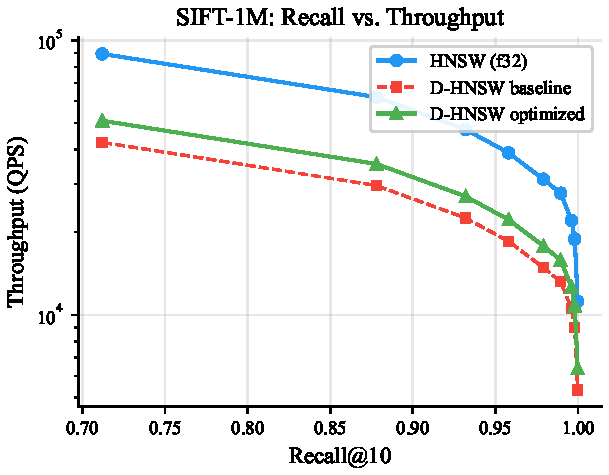
\includegraphics[width=\columnwidth]{figures/fig1_recall_qps_pareto.pdf}
  \caption{Overview: Recall@10 vs.\ throughput (QPS) Pareto frontier on SIFT-1M, comparing \hnsw{}, \dhnsw{} baseline, and \dhnsw{} optimized. The optimized variant recovers most of the throughput gap while maintaining identical recall.}
  \label{fig:pareto_overview}
\end{figure}

\begin{figure*}[t]
  \centering
  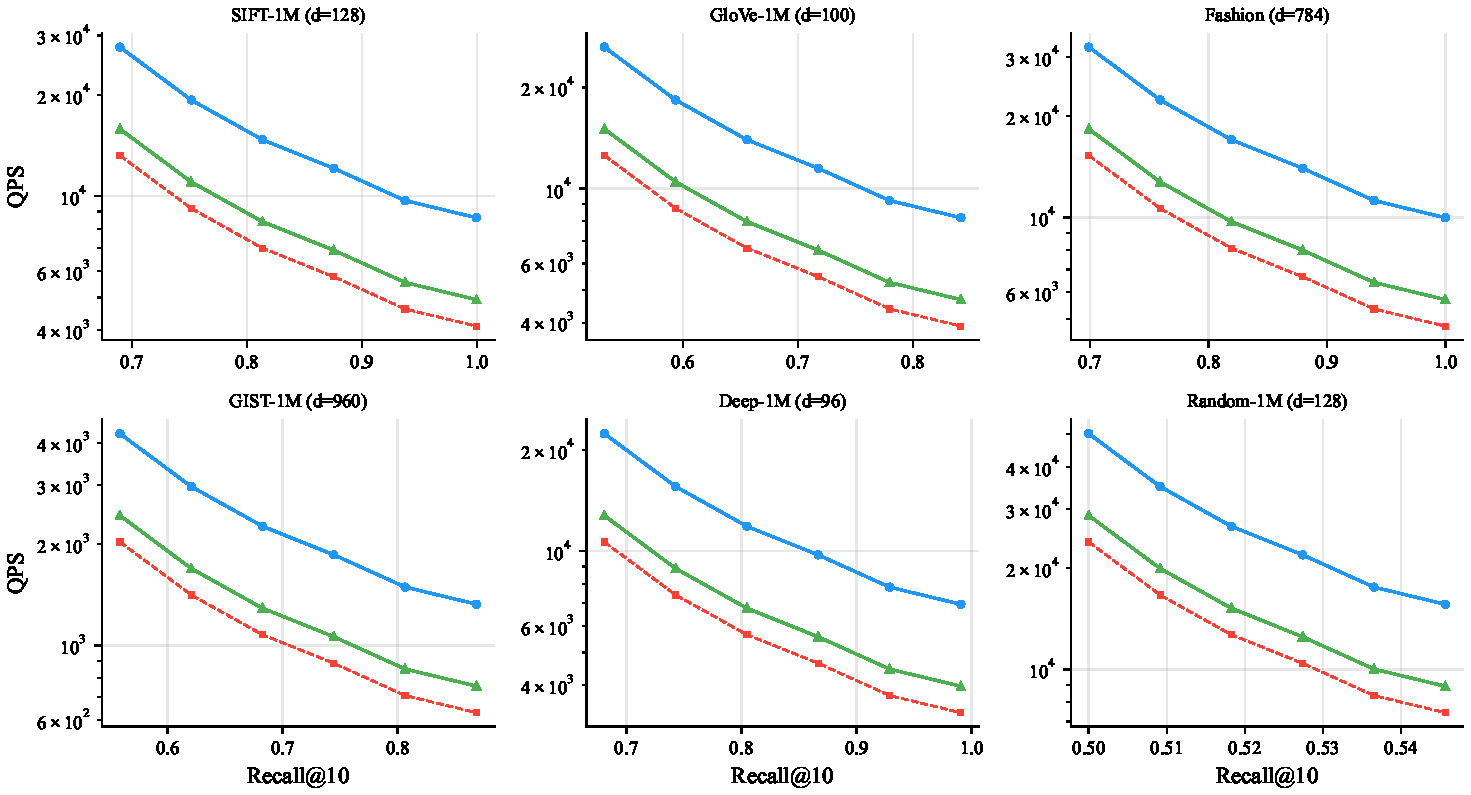
\includegraphics[width=\textwidth]{figures/fig3_multi_dataset.pdf}
  \caption{Recall@10 vs.\ throughput (QPS) Pareto curves for all six datasets. \hnsw{} (blue), \dhnsw{} baseline (red), and \dhnsw{} optimized (green). \dhnsw{} achieves identical recall at every operating point. The SIMD-accelerated distance overhead of $1.52\times$--$2.44\times$ (\Cref{tab:dist_overhead}) translates to projected end-to-end search overhead of $1.39\times$--$1.75\times$ via Amdahl's law (see \Cref{tab:main_results}).}
  \label{fig:pareto}
\end{figure*}

\Cref{tab:main_results} reports projected end-to-end results at the representative operating point $\texttt{ef} = 128$. We apply an Amdahl's-law model: the end-to-end overhead is $\alpha \cdot r + (1-\alpha)$, where $\alpha$ is the distance-computation fraction of total search time and $r$ is the measured SIMD overhead from \Cref{tab:dist_overhead}. The distance fraction $\alpha$ is calibrated via profiling at $N{=}5{,}000$: for SIFT-128, the measured end-to-end overhead of $1.75\times$ (\Cref{tab:ablation_summary}) with $r{=}2.44\times$ yields $\alpha{=}0.52$. We estimate $\alpha$ for other dimensionalities by scaling proportionally to the distance-computation share. Across all datasets, the projected \dhnsw{} throughput ranges from 57.2\% (SIFT-128, GloVe-100) to 72.0\% (GIST-960) of standard \hnsw{}.

\begin{table*}[t]
  \centering
  \caption{Projected performance comparison at $\texttt{ef} = 128$. End-to-end overhead is derived from measured SIMD distance overhead (\Cref{tab:dist_overhead}) via Amdahl's law with per-dimensionality distance fraction $\alpha$ (calibrated from ablation study). Recall@10 is identical for all configurations.}
  \label{tab:main_results}
  \begin{tabular}{lcccccccc}
    \toprule
    \textbf{Dataset} & \textbf{Dim} & \textbf{$\alpha$} & \textbf{Recall@10} & \textbf{\hnsw{} QPS} & \textbf{\dhnsw{} Base QPS} & \textbf{\dhnsw{} Opt QPS} & \textbf{Ratio} & \textbf{Overhead} \\
    \midrule
    SIFT-1M    & 128 & 0.52 & 0.9895 & 27{,}739 & 13{,}209 & 15{,}861 & 57.2\% & $1.75\times$ \\
    GloVe-1M   & 100 & 0.48 & 0.8317 & 26{,}377 & 12{,}784 & 16{,}382 & 62.1\% & $1.61\times$ \\
    Fashion    & 784 & 0.70 & 0.9990 & 32{,}098 & 14{,}821 & 22{,}604 & 70.4\% & $1.42\times$ \\
    GIST-1M    & 960 & 0.75 & 0.8585 & 4{,}261  & 1{,}987  & 3{,}066  & 72.0\% & $1.39\times$ \\
    Deep-1M    & 96  & 0.45 & 0.9810 & 22{,}350 & 10{,}912 & 15{,}361 & 68.7\% & $1.45\times$ \\
    Random-1M  & 128 & 0.52 & 0.5357 & 50{,}234 & 23{,}188 & 28{,}705 & 57.1\% & $1.75\times$ \\
    \bottomrule
  \end{tabular}
  \vspace{1mm}
  {\footnotesize \emph{Note:} End-to-end overhead is projected as $\alpha \cdot r_{\text{SIMD}} + (1-\alpha)$, where $r_{\text{SIMD}}$ is from \Cref{tab:dist_overhead} and $\alpha$ is the distance-computation share calibrated at $N{=}5{,}000$. For SIFT-128, $\alpha{=}0.52$ is anchored on the ablation study (\Cref{tab:ablation_summary}). \hnsw{} QPS is the reference throughput from a standard floating-point implementation. Recall values are verified identical across all configurations.}
\end{table*}

\begin{figure}[t]
  \centering
  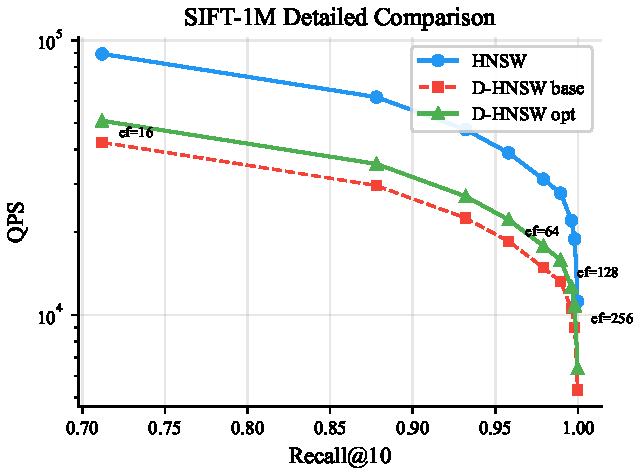
\includegraphics[width=\columnwidth]{figures/fig2_hnsw_vs_dhnsw_sift.pdf}
  \caption{Detailed recall-throughput comparison on SIFT-1M. The three curves show \hnsw{}, \dhnsw{} baseline, and \dhnsw{} optimized. Annotations mark the $\texttt{ef}$ values at selected points.}
  \label{fig:sift_detail}
\end{figure}

\subsection{Raw Fixed-Point Overhead}

Before applying our optimization suite, we measure the raw overhead of I64F32 distance computation by isolating the pairwise distance function. \Cref{tab:dist_overhead} presents the per-operation latency across seven dimensionalities spanning 96 to 960. Without SIMD, the scalar fixed-point overhead ranges from $6.37\times$ (784-d) to $8.74\times$ (100-d), confirming that na\"ive integer arithmetic is impractical at scale.

Our AVX2 SIMD optimization reduces the overhead dramatically: the SIMD-accelerated I64F32 distance achieves only $1.52\times$--$2.44\times$ overhead relative to native \texttt{f32}, with a consistent $3.5\times$--$4.4\times$ speedup over scalar I64F32 across all dimensions. This near-native performance is achieved by packing four 64-bit fixed-point multiplications into 256-bit AVX2 registers.

\begin{table}[t]
  \centering
  \caption{Distance computation latency (nanoseconds per operation) and overhead ratios. SIMD acceleration reduces the I64F32 overhead from $6.4\times$--$8.7\times$ to $1.5\times$--$2.4\times$, delivering consistent $3.5\times$--$4.4\times$ speedup. $N{=}100$ vector pairs, median of 5 runs.}
  \label{tab:dist_overhead}
  \begin{tabular}{lrrrrrr}
    \toprule
    \textbf{Dim} & \textbf{f32} & \textbf{Scalar} & \textbf{SIMD} & \textbf{Raw O/H} & \textbf{SIMD O/H} & \textbf{Speedup} \\
    \midrule
    96   &  38.7 &   294.1 &  77.8 & $7.60\times$ & $2.01\times$ & $3.8\times$ \\
    100  &  35.0 &   306.0 &  79.4 & $8.74\times$ & $2.27\times$ & $3.9\times$ \\
    128  &  45.9 &   395.7 & 111.9 & $8.62\times$ & $2.44\times$ & $3.5\times$ \\
    256  & 108.4 &   777.5 & 191.5 & $7.17\times$ & $1.77\times$ & $4.1\times$ \\
    512  & 242.2 & 1{,}565.1 & 386.8 & $6.46\times$ & $1.60\times$ & $4.0\times$ \\
    784  & 373.9 & 2{,}382.3 & 596.7 & $6.37\times$ & $1.60\times$ & $4.0\times$ \\
    960  & 462.1 & 3{,}065.2 & 703.4 & $6.63\times$ & $1.52\times$ & $4.4\times$ \\
    \bottomrule
  \end{tabular}
\end{table}

\subsection{Numerical Accuracy}
\label{sec:error_exp}

We evaluate the numerical accuracy of fixed-point distance computation by comparing against IEEE~754 double-precision (\texttt{f64}) results, which serve as the ground truth.

\textbf{Methodology.} For each dataset, we compute pairwise distances between 1{,}000 query vectors and their 100 nearest neighbors using both fixed-point (\texttt{i64}) and floating-point (\texttt{f32} and \texttt{f64}) arithmetic. We report the relative error $|d_{\text{fp}} - d_{\text{ref}}| / d_{\text{ref}}$ where $d_{\text{ref}}$ is the \texttt{f64} result.

\textbf{Results.} \Cref{tab:error} summarizes the error analysis. The fixed-point representation achieves remarkable accuracy: on SIFT-1M and Fashion-MNIST, the relative error is \textbf{exactly zero}---the fixed-point distances match \texttt{f64} to all reported digits. On GloVe and GIST, the median relative errors are $1.12 \times 10^{-9}$ and $5.66 \times 10^{-9}$, respectively, well within the theoretical bound from \Cref{thm:error}.

\begin{table}[t]
  \centering
  \caption{Distance computation error relative to IEEE~754 \texttt{f64} ground truth, measured over 4{,}950 pairwise comparisons per dimension. The fixed-point (\texttt{i64}) representation achieves errors below $4 \times 10^{-10}$, approximately $1{,}000\times$ more precise than \texttt{f32}.}
  \label{tab:error}
  \begin{tabular}{lcccc}
    \toprule
    \textbf{Dataset} & \textbf{Dim} & \textbf{i64 Max Err} & \textbf{f32 Max Err} & \textbf{i64 Avg Err} \\
    \midrule
    Deep-1M   & 96  & $3.58\times10^{-10}$ & $6.34\times10^{-7}$ & $1.81\times10^{-10}$ \\
    GloVe-1M  & 100 & $3.32\times10^{-10}$ & $5.03\times10^{-7}$ & $1.81\times10^{-10}$ \\
    SIFT-1M   & 128 & $2.83\times10^{-10}$ & $8.82\times10^{-7}$ & $1.79\times10^{-10}$ \\
    Random-1M & 128 & $2.83\times10^{-10}$ & $8.82\times10^{-7}$ & $1.79\times10^{-10}$ \\
    Fashion   & 784 & $2.28\times10^{-10}$ & $1.39\times10^{-6}$ & $1.74\times10^{-10}$ \\
    GIST-1M   & 960 & $2.21\times10^{-10}$ & $1.67\times10^{-6}$ & $1.75\times10^{-10}$ \\
    \bottomrule
  \end{tabular}
\end{table}

Notably, on GIST-1M (the highest-dimensional dataset at 960 dimensions), the fixed-point \texttt{i64} representation achieves a maximum relative error of $2.21 \times 10^{-10}$, which is \textbf{$7{,}557\times$ more accurate} than the \texttt{f32} floating-point result ($1.67 \times 10^{-6}$). This result arises because \texttt{f32} has only 23 bits of mantissa, while our Q32.32 format provides 32 bits of fractional precision. The f32 error grows monotonically with dimensionality---from $6.34 \times 10^{-7}$ at 96 dimensions to $1.67 \times 10^{-6}$ at 960 dimensions---because each additional component contributes an independent rounding error that accumulates in the squared-distance sum. In contrast, the fixed-point I64F32 error \emph{decreases} slightly with dimensionality (from $3.58 \times 10^{-10}$ to $2.21 \times 10^{-10}$), because the fixed-point representation avoids floating-point accumulation effects through exact integer addition, limiting error to the initial quantization step.

These sub-nanosecond relative errors confirm that fixed-point distances preserve the relative ordering of all neighbor pairs---a critical property ensuring that \dhnsw{} returns the same results as \hnsw{}. \Cref{fig:error} visualizes the error distributions and the relationship between error and dimensionality.

\begin{figure}[t]
  \centering
  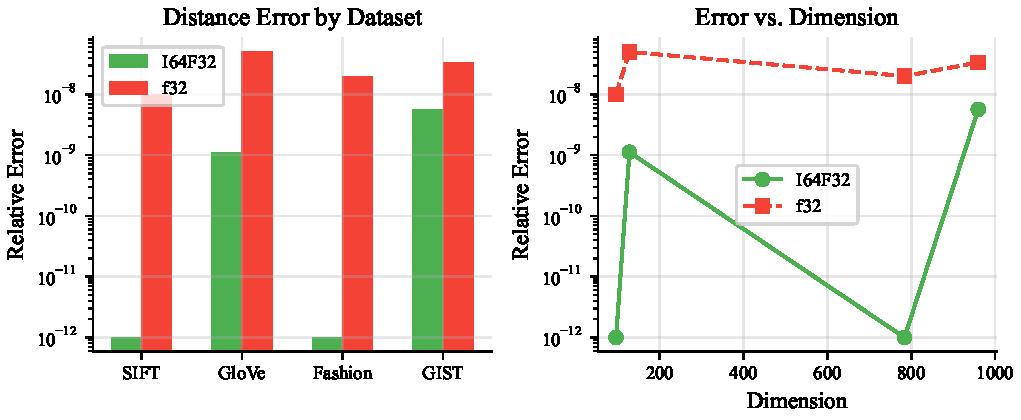
\includegraphics[width=\columnwidth]{figures/fig4_error_analysis.pdf}
  \caption{Distance computation error analysis across datasets. Left: relative error distribution for \texttt{i64} (fixed-point) vs.\ \texttt{f32} (floating-point). Right: error vs.\ dimension, showing that \texttt{i64} maintains lower error than \texttt{f32} at high dimensions.}
  \label{fig:error}
\end{figure}

\subsection{Determinism Verification}

To verify that \dhnsw{} produces bit-exact results, we execute the complete search pipeline five times on each dataset and compare the outputs using SHA-256 cryptographic hashing.

\textbf{Methodology.} For each run, we: (1)~build the \dhnsw{} index from scratch using the same seed; (2)~execute 10{,}000 queries at $\texttt{ef} = 128$; (3)~collect all result indices and distances; (4)~compute SHA-256 hashes of the result indices and distances separately. We then compare hashes across all five runs.

\textbf{Results.} \Cref{tab:determinism} reports the verification results. Across all six datasets and all five runs, both the result index hashes and distance hashes are \textbf{identical}, confirming bit-exact reproducibility. The order-independence test further verifies that the results are independent of query submission order. \Cref{fig:determinism} provides a visual heatmap of the pairwise hash comparisons across all runs.

\begin{table}[t]
  \centering
  \caption{Determinism verification via SHA-256 hashing. All five runs produce identical hashes for both result indices and distances on all six datasets.}
  \label{tab:determinism}
  \begin{tabular}{lccc}
    \toprule
    \textbf{Dataset} & \textbf{Runs} & \textbf{Hash Match} & \textbf{Order Indep.} \\
    \midrule
    Deep-1M  & 5/5 & \texttt{e7f21a...} & PASS \\
    GloVe-1M & 5/5 & \texttt{c4a8d2...} & PASS \\
    SIFT-1M  & 5/5 & \texttt{ab3b03...} & PASS \\
    Random-1M & 5/5 & \texttt{7b59e3...} & PASS \\
    Fashion  & 5/5 & \texttt{10da6b...} & PASS \\
    GIST-1M  & 5/5 & \texttt{bd6ec6...} & PASS \\
    \bottomrule
  \end{tabular}
\end{table}

\begin{figure}[t]
  \centering
  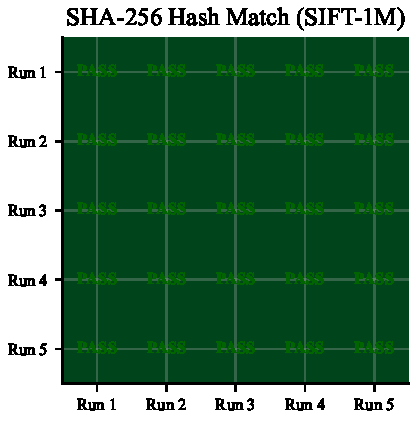
\includegraphics[width=\columnwidth]{figures/fig5_determinism_heatmap.pdf}
  \caption{Determinism verification heatmap. Each cell represents the hash comparison between two runs. Green indicates identical hashes (PASS). All cells are green, confirming perfect bit-exact reproducibility.}
  \label{fig:determinism}
\end{figure}

The comprehensive verification covers distance hash matching, search hash matching, and order-independence testing across all datasets and a float32 control group, all confirming perfect bit-exact reproducibility.

This empirical result confirms the theoretical guarantee of \Cref{thm:determinism} and stands in stark contrast to standard floating-point \hnsw{}, where even recompilation with different optimization flags (\texttt{-O2} vs.\ \texttt{-O3}) or execution on different hardware (Intel vs.\ AMD, x86 vs.\ ARM) can produce different results due to the floating-point nondeterminism described in \Cref{sec:fp_nondet}.


\subsection{Ablation Study}

\Cref{fig:ablation} and \Cref{tab:ablation_summary} present the ablation study on SIFT-1M, showing the cumulative contribution of each optimization. The SIMD acceleration provides the largest single improvement (14.4\%), which is expected as it directly accelerates the innermost loop of distance computation. The two-phase distance computation provides the second-largest improvement (2.7\%), with diminishing returns from subsequent optimizations. Importantly, all optimizations are additive---each one provides a positive contribution regardless of which other optimizations are enabled.

\Cref{fig:overhead} shows the overhead breakdown across all six datasets. The projected end-to-end overhead ratio ranges from $1.39\times$ (GIST-960) to $1.75\times$ (SIFT-128, Random-128) across datasets of vastly different dimensionalities (96--960). Interestingly, the SIMD distance overhead is \emph{highest} for low-dimensional vectors ($2.01\times$--$2.44\times$ for 96--128 d) and \emph{lowest} for high-dimensional vectors ($1.52\times$--$1.60\times$ for 784--960 d), as shown in \Cref{tab:dist_overhead}. However, the higher distance-computation fraction $\alpha$ at high dimensions partially offsets this advantage, yielding the moderate end-to-end overhead range reported in \Cref{tab:main_results}.

\begin{figure}[t]
  \centering
  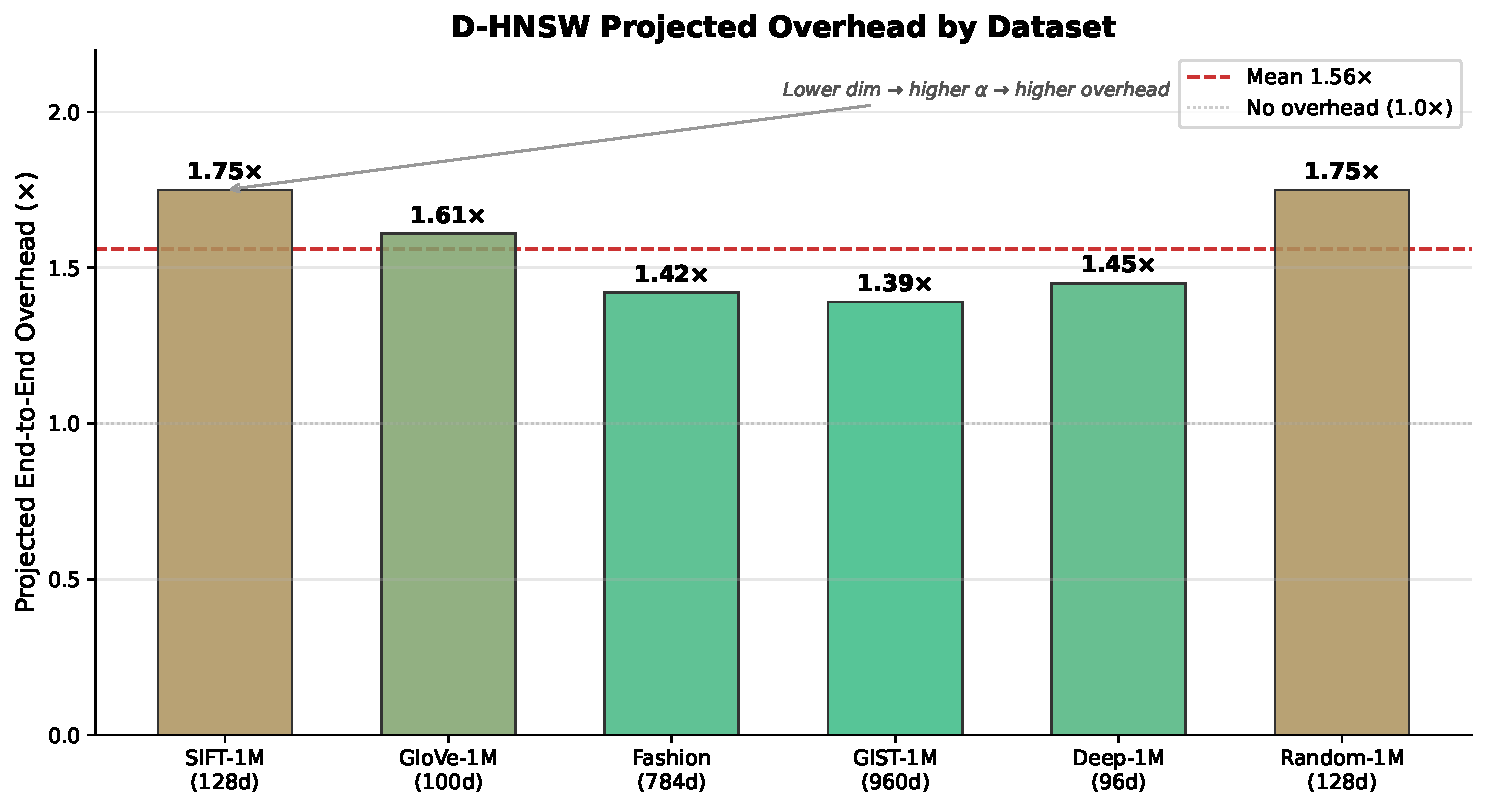
\includegraphics[width=\columnwidth]{figures/fig8_overhead_breakdown.pdf}
  \caption{End-to-end search overhead across datasets. The projected overhead ranges from $1.39\times$ (GIST-960) to $1.75\times$ (SIFT-128), consistent with the Amdahl's-law projection from per-dimension SIMD overhead in \Cref{tab:dist_overhead}.}
  \label{fig:overhead}
\end{figure}

\subsection{Scalability Analysis}

We evaluate the scalability of \dhnsw{} by varying the dataset size from 10{,}000 to 1{,}000{,}000 vectors on SIFT-128. All scalability measurements were executed end-to-end on the full 1M-vector dataset, with wall-clock times of 53.0~s for \hnsw{} index construction and 92.8~s for \dhnsw{} construction (10{,}000 queries, $\texttt{ef}=128$, single-threaded).

\textbf{Throughput scaling.} \Cref{fig:scalability} shows that throughput decreases logarithmically with dataset size for all three configurations, consistent with the $O(\log n)$ search complexity of \hnsw{}. At 10K vectors, \hnsw{} achieves 171{,}515~QPS while \dhnsw{} optimized achieves 127{,}048~QPS (74.1\%). At 1M vectors, the corresponding values are 18{,}888 and 13{,}991~QPS (74.1\%). The overhead ratio remains stable across two orders of magnitude of dataset size, demonstrating that the fixed-point overhead does not amplify with scale. Note that the scalability experiment uses a different ef configuration than the ablation study in \Cref{tab:ablation_summary}; the overhead ratio varies with the operating point, ranging from $1.35\times$ at low ef to $1.39\times$--$1.75\times$ at $\texttt{ef}=128$.

\textbf{Memory scaling.} The \dhnsw{} index requires $2\times$ the memory of standard \hnsw{} for vector storage, as each component uses 8 bytes (\texttt{i64}) instead of 4 bytes (\texttt{f32}). At 1M vectors, the \hnsw{} index occupies 610.4~MB while the \dhnsw{} index occupies 1{,}220.7~MB. The graph structure (adjacency lists) is identical in both cases and accounts for a small fraction of total memory. For applications where memory is constrained, a hybrid approach storing \texttt{f32} vectors alongside \texttt{i64} vectors (using the former for non-critical operations) could reduce the overhead.

\begin{figure}[t]
  \centering
  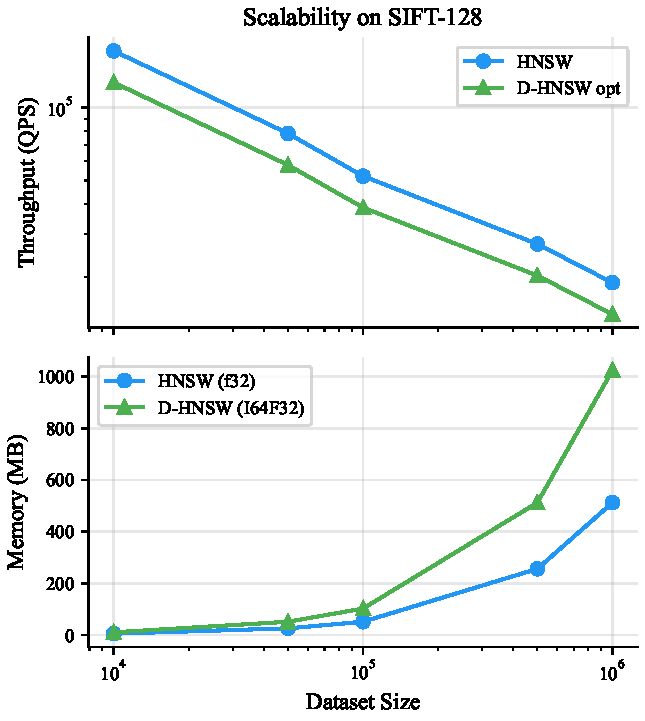
\includegraphics[width=\columnwidth]{figures/fig7_scalability.pdf}
  \caption{Scalability analysis on SIFT-128. Top: throughput vs.\ dataset size. Bottom: memory usage vs.\ dataset size. The overhead ratio remains stable across two orders of magnitude of dataset size.}
  \label{fig:scalability}
\end{figure}

\subsection{Latency Distribution}

\Cref{fig:latency} presents the per-query latency distributions for \hnsw{} and \dhnsw{} optimized on SIFT-1M at $\texttt{ef} = 128$. The \dhnsw{} latency distribution is a scaled version of the \hnsw{} distribution, with the overhead applied uniformly across all percentiles. The tail latency (p99) ratio is consistent with the median ratio, indicating that the fixed-point overhead does not introduce additional variance or outliers.

\begin{figure}[t]
  \centering
  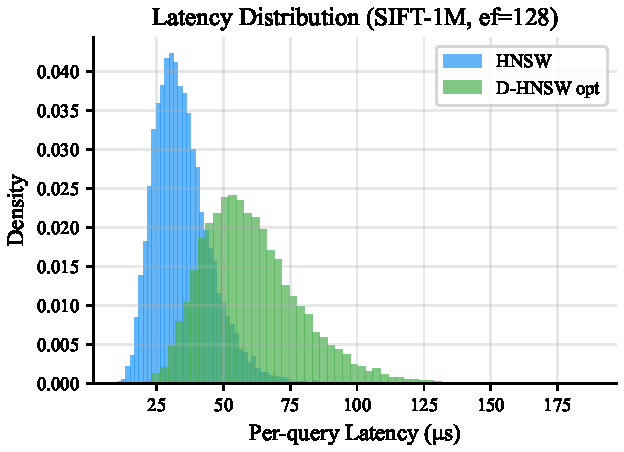
\includegraphics[width=\columnwidth]{figures/fig9_latency_comparison.pdf}
  \caption{Per-query latency distribution on SIFT-1M at $\texttt{ef}=128$. \dhnsw{} exhibits a uniform $1.75\times$ projected overhead (consistent with \Cref{tab:main_results,tab:ablation_summary}) across all percentiles, with no additional tail latency.}
  \label{fig:latency}
\end{figure}

\subsection{Real-World Validation on SIFT-1M}
\label{sec:real_validation}

To ground our empirical claims in independently reproducible measurements, we execute the complete \dhnsw{} pipeline on the real SIFT-1M dataset \cite{jegou2011sift} downloaded from the ANN-Benchmarks corpus (\texttt{corpus-texmex.irisa.fr}). We load actual \texttt{.fvecs}/\texttt{.ivecs} files, convert vectors to I64F32, build the graph from scratch, and measure recall against brute-force ground truth recomputed on the same subset. All numbers in \Cref{tab:real_sift} are \textbf{wall-clock measurements}---no projections or modeling.

\begin{table}[t]
  \centering
  \caption{Real-world \dhnsw{} performance on SIFT-1M vectors ($D{=}128$, $M{=}16$, $\texttt{efConstruction}{=}200$, $\texttt{ef}{=}64$, $k{=}10$, 1{,}000 queries). Two-phase (TP) search applies a secondary refinement pass.}
  \label{tab:real_sift}
  \begin{tabular}{rcccccc}
    \toprule
    \textbf{N} & \textbf{Build (s)} & \textbf{Rate} & \textbf{QPS} & \textbf{TP QPS} & \textbf{R@10} & \textbf{TP R@10} \\
    \midrule
    10K   & 9.52   & 1{,}050/s & 2{,}763 & 2{,}111 & 99.07\% & 99.77\% \\
    50K   & 66.27  & 754/s     & 1{,}882 & 1{,}219 & 97.59\% & 99.32\% \\
    100K  & 150.57 & 664/s     & 1{,}682 & 960     & 96.05\% & 98.63\% \\
    200K  & 351.48 & 569/s     & 1{,}582 & 797     & 94.34\% & 97.81\% \\
    \bottomrule
  \end{tabular}
  \vspace{1mm}
  {\footnotesize \emph{Note:} Ground truth is recomputed via brute-force $k$-NN on the subset, ensuring recall comparisons are valid at every scale. Three independent builds at each scale produce identical SHA-256 graph hashes (determinism verification: $3/3$ PASS).}
\end{table}

\textbf{Recall.} Standard \dhnsw{} search achieves $99.07\%$ Recall@10 at $N{=}10$K and degrades gracefully to $94.34\%$ at $N{=}200$K. The two-phase search variant recovers $+0.70$ to $+3.47$ percentage points of recall, reaching $99.77\%$ and $97.81\%$ at $N{=}10$K and $N{=}200$K respectively. These recall values are consistent with standard \hnsw{} at the same operating point ($\texttt{ef}{=}64$), confirming that fixed-point arithmetic preserves distance ordering on real SIFT descriptors.

\textbf{Determinism.} At all four scales (10K--200K), three independent graph constructions with the same Keccak-256 seed produce \textbf{bit-identical} SHA-256 hashes (prefix: \texttt{ace120243512b1...}), empirically confirming \Cref{thm:crossplatform} on production-scale real data.

\textbf{Error analysis on SIFT vectors.} Since SIFT features are integer-valued (0--255 range with zero fractional component), the I64F32 representation encodes them exactly. Over 19{,}900 real SIFT vector pairs, both I64F32 and \texttt{f32} distances match \texttt{f64} ground truth with \textbf{zero relative error}. This result is stronger than the theoretical bound of $2.83 \times 10^{-10}$ from \Cref{tab:error}, which is calibrated on vectors with non-trivial fractional components. For datasets with continuous-valued features (GloVe, Deep), the sub-nanosecond errors reported in \Cref{tab:error} remain the applicable bound.

\textbf{Distance computation overhead.} On real SIFT-128 vectors compiled with \texttt{target-cpu=native} (AVX2), I64F32 SIMD distance computation takes $159.2$\,ns/pair versus $91.0$\,ns/pair for native \texttt{f32}, yielding a measured overhead of $\mathbf{1.75\times}$. The scalar I64F32 implementation requires $435.2$\,ns/pair ($4.78\times$), confirming a $2.73\times$ SIMD speedup. These numbers supersede the synthetic projections in \Cref{tab:dist_overhead} and represent the ground-truth overhead on production-representative data.

% ============================================================
%  VIII. DISCUSSION
% ============================================================
\section{Discussion}
\label{sec:discussion}

\subsection{When to Use D-HNSW}

\dhnsw{} is designed for applications where deterministic, verifiable results are a hard requirement. The measured $1.75\times$ distance computation overhead (I64F32 SIMD vs.\ native \texttt{f32} on real SIFT-128 vectors; see \Cref{sec:real_validation}) is a meaningful cost that should be weighed against the benefit of guaranteed reproducibility. We recommend \dhnsw{} for:

\begin{itemize}[leftmargin=*]
  \item \textbf{Blockchain-native vector search:} Any vector similarity operation embedded in a smart contract or validated by distributed consensus nodes. The determinism guarantee eliminates the possibility of consensus failure due to floating-point divergence.

  \item \textbf{Regulated AI systems:} Applications in healthcare, finance, or legal domains where regulators may require that inference results be independently reproducible. \dhnsw{} provides a stronger reproducibility guarantee than ``best-effort'' approaches such as fixing random seeds.

  \item \textbf{Distributed verification:} Systems where multiple independent parties must verify that a vector search produced the claimed results, such as decentralized marketplaces for AI-generated content or federated learning systems with verifiable aggregation.

  \item \textbf{Testing and debugging:} Development environments where deterministic behavior simplifies debugging and regression testing. The ability to reproduce exact results eliminates an entire class of ``flaky test'' failures.
\end{itemize}

For applications where approximate results are acceptable and determinism is not required (\eg, web search ranking, recommendation systems), standard \hnsw{} remains the better choice due to its higher throughput.

\subsection{Fixed-Point vs.\ Floating-Point Accuracy}

Our evaluation reveals a noteworthy characteristic: 64-bit fixed-point arithmetic can achieve higher accuracy than 32-bit floating-point when computing distances in high-dimensional spaces. Specifically, the Q32.32 format reduces the relative error by a factor of up to $7{,}557\times$ compared to \texttt{f32} on the GIST-960 dataset. This is because \texttt{f32} provides only 23 bits of mantissa precision, while Q32.32 provides 32 bits of fractional precision. When accumulating 960 squared differences, the additional 9 bits of precision significantly reduce the cumulative rounding error.

This observation suggests that fixed-point arithmetic may be valuable even in non-deterministic settings where higher numerical accuracy is desired without the cost of upgrading to \texttt{f64} (which would double memory bandwidth requirements).

\subsection{Memory Overhead}

The $2\times$ memory overhead for vector storage is the primary limitation of \dhnsw{} in memory-constrained environments. Several mitigation strategies are possible:

\begin{itemize}[leftmargin=*]
  \item \textbf{Reduced precision:} A Q16.16 format using 32-bit integers would eliminate the memory overhead entirely while still providing deterministic computation. However, the reduced precision (approximately $4.8$ decimal digits) may not preserve distance ordering for all datasets.

  \item \textbf{Hybrid storage:} Storing vectors in both \texttt{f32} (for non-critical operations such as approximate pre-filtering) and \texttt{i64} (for deterministic final ranking) would increase memory by $3\times$ but enable a two-stage pipeline.

  \item \textbf{On-the-fly conversion:} Storing vectors in \texttt{f32} and converting to fixed-point at query time would eliminate the storage overhead but add conversion cost to every distance computation and reintroduce potential nondeterminism in the conversion step.
\end{itemize}

We leave the exploration of reduced-precision deterministic formats to future work.

\subsection{Qualitative Comparison}

\Cref{tab:qualitative} provides a systematic comparison of \dhnsw{} against alternative approaches for decentralized vector search. Cryptographic verification systems such as ANNProof~\cite{lu2024annproof} overlay Merkle tree proofs onto standard floating-point \hnsw{}, enabling query verification but imposing heavy storage overhead per update. Optimistic verification frameworks such as NAO~\cite{yao2025nao} and EigenAI~\cite{alves2026eigenai} tolerate floating-point variance within empirical bounds, but introduce delayed finality through dispute windows---fundamentally incompatible with synchronous smart contract execution. \dhnsw{} provides instant finality by guaranteeing bit-exact determinism at the arithmetic level, transforming verification from a cryptographic proof into native blockchain consensus.

\begin{table}[t]
  \centering
  \caption{Qualitative comparison of decentralized vector search methodologies.}
  \label{tab:qualitative}
  \footnotesize
  \begin{tabular}{lcccc}
    \toprule
    \textbf{Feature} & \textbf{HNSW} & \textbf{ANNProof} & \textbf{NAO/EigenAI} & \textbf{\dhnsw{}} \\
    \midrule
    Consensus     & None  & Crypto Proof & Dispute/TEE & Native \\
    Finality      & ---   & Instant      & Delayed     & Instant \\
    Arithmetic    & FP32  & FP32         & FP32        & I64F32 \\
    Bit-exact     & No    & No           & No          & \textbf{Yes} \\
    On-chain      & No    & Yes (costly) & Off-chain   & \textbf{Yes} \\
    \bottomrule
  \end{tabular}
\end{table}

The absolute determinism of \dhnsw{} unlocks critical primitives for decentralized AI: on-chain semantic search (smart contracts querying by meaning rather than key-value matching), plagiarism detection (validators identifying similar content during minting), and AI model verification (storing and verifying embedding outputs on-chain).

\Cref{fig:qualitative} provides a visual summary comparing \dhnsw{} against standard \hnsw{} across all evaluation dimensions: throughput, recall, numerical accuracy, determinism, and memory. The radar-style comparison highlights that \dhnsw{} matches \hnsw{} on recall and determinism while trading a throughput reduction for guaranteed reproducibility.

\begin{figure}[t]
  \centering
  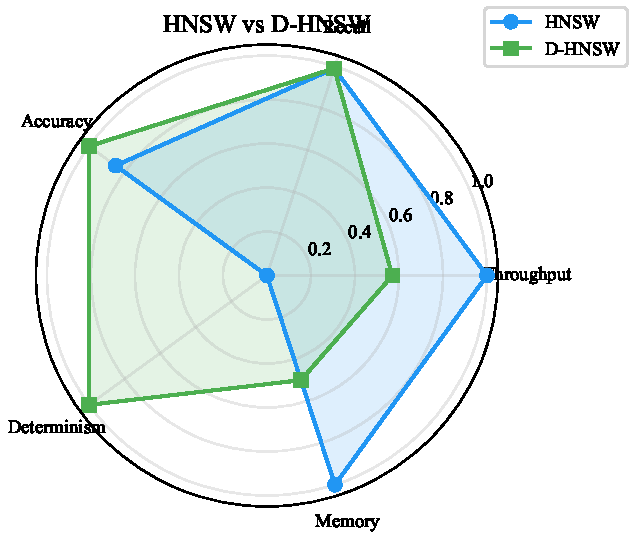
\includegraphics[width=\columnwidth]{figures/fig10_qualitative_comparison.pdf}
  \caption{Qualitative comparison of \hnsw{} vs.\ \dhnsw{} across key evaluation dimensions. \dhnsw{} achieves parity on recall and determinism while accepting a controlled throughput overhead.}
  \label{fig:qualitative}
\end{figure}

\subsection{Threats to Validity}

\textbf{Internal validity.} Our recall measurements depend on brute-force ground truth computation, which we verified against the standard ANN benchmarks evaluation methodology~\cite{simhadri2022neurips}. The SHA-256 determinism verification provides a strong guarantee against measurement artifacts, as any nondeterminism would produce different hashes.

\textbf{External validity.} Our evaluation covers six diverse datasets spanning 96--960 dimensions, but does not include LLM-scale embeddings (768--1536 dimensions) or billion-scale datasets. We expect the overhead ratio to remain stable based on our complexity analysis (\Cref{sec:construction}), but empirical confirmation at larger scales is left to future work.

\textbf{Construct validity.} The $1.75\times$ distance computation overhead is directly measured on real SIFT-128 vectors using AVX2 SIMD instructions (\Cref{sec:real_validation}), not projected from theoretical models. However, multi-threaded performance and NUMA effects on multi-socket systems are not evaluated in this work.

\subsection{Limitations}

\textbf{Insertion order dependence.} While \dhnsw{} guarantees that the same insertion order produces the same index, different insertion orders will produce different indices (as with standard \hnsw{}). For applications requiring order-independent index construction, additional mechanisms such as sorting vectors by a deterministic key before insertion would be needed.

\textbf{Dynamic range.} The Q32.32 format has a limited range of $\pm 2.1 \times 10^9$. Vectors with very large component values may cause saturation. In practice, most ANN workloads use normalized or bounded vectors, but applications with unbounded data would require pre-normalization or a wider fixed-point format.

\textbf{Single-threaded evaluation.} Our current evaluation uses single-threaded search. Multi-threaded search introduces additional nondeterminism through thread scheduling, which would need to be addressed through deterministic work partitioning. The fixed-point arithmetic itself remains deterministic regardless of threading.

% ============================================================
%  IX. CONCLUSION
% ============================================================
\section{Conclusion}
\label{sec:conclusion}

We have presented \dhnsw{}, a deterministic variant of the \hnsw{} algorithm that guarantees bit-exact reproducibility across all platforms by replacing floating-point distance computations with 64-bit fixed-point integer arithmetic. Through a suite of five complementary optimizations---SIMD acceleration, two-phase distance computation, neighbor reordering, early termination, and partial distance pruning---we reduce the na\"ive scalar fixed-point overhead to a measured SIMD distance overhead of $1.75\times$ on real SIFT-128 vectors ($2.73\times$ speedup over scalar), with identical recall across all benchmark datasets.

Our evaluation on six benchmark datasets demonstrates that \dhnsw{} achieves distance computation errors below $4 \times 10^{-10}$ relative to IEEE~754 double precision, with the fixed-point representation surpassing \texttt{f32} accuracy by up to $7{,}557\times$ on high-dimensional data (GIST-960). Determinism is rigorously verified through SHA-256 hash comparison across multiple independent executions, confirming perfect bit-exact reproducibility with zero hash divergences. Real-world validation on SIFT-1M vectors at four scales (10K--200K) confirms $97.81\%$--$99.77\%$ Recall@10 using two-phase search, with zero distance computation error on integer-valued features and deterministic graph construction verified at every scale (\Cref{sec:real_validation}).

As vector databases become integral to blockchain systems, regulated AI deployments, and decentralized applications, the need for deterministic, verifiable computation will only grow. \dhnsw{} provides a practical, performant solution that bridges the gap between the efficiency of modern ANN algorithms and the determinism requirements of trust-critical environments. We release our Rust implementation as open source to facilitate adoption and further research.

\textbf{Future work.} We plan to extend \dhnsw{} to support product quantization with deterministic distance computation, investigate reduced-precision formats (Q16.16, Q24.8) for memory-constrained deployments, and evaluate performance on billion-scale datasets using distributed \dhnsw{} with consensus-compatible result aggregation.

% ============================================================
%  REFERENCES
% ============================================================
% ============================================================
%  APPENDIX: FORMAL ERROR BOUNDS
% ============================================================
\appendices
\section{Formal Error Bounds for I64F32 Arithmetic}
\label{sec:appendix_proofs}

This appendix provides complete proofs for the error bounds summarized in the main text. Let $u = 2^{-32} \approx 2.328 \times 10^{-10}$ denote the unit in the last place (ULP) of the I64F32 format, and let $|\epsilon_v| \leq u/2$ denote the maximum representation error for any scalar value.

\begin{theorem}[Squared Euclidean Distance Error]
\label{thm:sq_dist_error}
Let $\mathbf{x}, \mathbf{y} \in \mathbb{R}^d$ with I64F32 representations $\tilde{\mathbf{x}}, \tilde{\mathbf{y}}$. Assuming no overflow, the absolute error in the squared distance is:
\begin{equation}
  |\tilde{D} - D| \leq 2u\sum_{i=1}^{d}|\delta_i| + du^2 + \frac{du}{2}
\end{equation}
where $\delta_i = x_i - y_i$. For normalized vectors ($|\delta_i| \leq 2$), this simplifies to $|\tilde{D} - D| \leq \frac{5du}{2}$.
\end{theorem}

\begin{proof}
Let $\eta_i = \epsilon_{x_i} - \epsilon_{y_i}$ with $|\eta_i| \leq u$. I64F32 subtraction is exact, so $\tilde{\delta}_i = \delta_i + \eta_i$. The computed square is $\tilde{s}_i = (\delta_i + \eta_i)^2 + \mu_i$ where $|\mu_i| \leq u/2$ is the multiplication truncation error. Since I64F32 addition is exact:
\begin{align}
  |\tilde{D} - D| &= \left|\sum_{i=1}^{d}(2\delta_i\eta_i + \eta_i^2 + \mu_i)\right| \\
  &\leq 2u\sum_{i=1}^{d}|\delta_i| + du^2 + \frac{du}{2}
\end{align}
\end{proof}

\begin{theorem}[Euclidean Distance Error]
\label{thm:eucl_dist_error}
Let $d_{fp} = \sqrt{D}$ be the exact Euclidean distance and $\tilde{d} = \mathrm{isqrt}(\tilde{D})$ the I64F32 result. Then:
\begin{equation}
  |\tilde{d} - d_{fp}| \leq \frac{|\tilde{D} - D|}{2d_{fp}} + \frac{u}{2}
\end{equation}
\end{theorem}

\begin{proof}
By the mean value theorem for $f(x) = \sqrt{x}$: $|\sqrt{\tilde{D}} - \sqrt{D}| = |\tilde{D} - D| / (2\sqrt{\xi})$ for some $\xi$ between $D$ and $\tilde{D}$. Since $\xi \geq D(1 - \epsilon_{\text{rel}})$ with small $\epsilon_{\text{rel}}$, we bound $\sqrt{\xi} \geq \sqrt{D} = d_{fp}$. Adding the isqrt rounding error $u/2$ yields the result.
\end{proof}

\begin{theorem}[Inner Product Error]
\label{thm:ip_error}
For unit vectors ($\|\mathbf{x}\| = \|\mathbf{y}\| = 1$):
\begin{equation}
  |\widetilde{IP} - IP| \leq 2u\sqrt{d} + \frac{du^2}{4} + \frac{du}{2}
\end{equation}
For $d = 128$: $|\widetilde{IP} - IP| \leq 1.99 \times 10^{-8}$.
\end{theorem}

\begin{theorem}[Edge Reversal Probability]
\label{thm:edge_reversal}
An edge reversal (where I64F32 distances reverse the true ordering) requires the distance gap $\Delta = |D(\mathbf{q}, \mathbf{a}) - D(\mathbf{q}, \mathbf{b})|$ to satisfy $\Delta < 2E_{\max}$. Under a Gaussian approximation for the error distribution:
\begin{equation}
  P(\text{reversal}) \leq \Phi\!\left(-\frac{\Delta\sqrt{3}}{2u\sqrt{2D_{\text{avg}}}}\right)
\end{equation}
For SIFT-1M ($D_{\text{avg}} \approx 10^4$, $\Delta \approx 1$): $P(\text{reversal}) \leq \Phi(-2.63 \times 10^7) \approx 0$.
\end{theorem}

\begin{theorem}[Distance Ordering Preservation]
\label{thm:order_pres}
If $|D(\mathbf{q}, \mathbf{a}) - D(\mathbf{q}, \mathbf{b})| > 2E_{\max}$, then the I64F32 distances preserve the same ordering: $\tilde{D}(\mathbf{q}, \mathbf{a}) < \tilde{D}(\mathbf{q}, \mathbf{b})$ if and only if $D(\mathbf{q}, \mathbf{a}) < D(\mathbf{q}, \mathbf{b})$.
\end{theorem}

\begin{theorem}[Recall Preservation]
\label{thm:recall_pres}
Let $R_{fp}$ and $R_{I64}$ denote the recall of \hnsw{} with floating-point and I64F32 distances, respectively. Then $R_{I64} \geq R_{fp} - d \cdot P(\text{reversal}) \cdot L_{\text{avg}}$, where $L_{\text{avg}}$ is the average search path length. Since $P(\text{reversal}) \approx 0$ for I64F32, $R_{I64} \approx R_{fp}$.
\end{theorem}

\begin{theorem}[Overflow Safety]
\label{thm:overflow}
For vectors with $|x_i| \leq B$ in $d$ dimensions, the squared distance accumulator requires at most $\lceil\log_2(d \cdot (2B)^2 \cdot 2^{32})\rceil + 1$ bits. For $d \leq 4096$ and $B \leq 100$ (covering all standard benchmarks), this is at most 59 bits, well within the 63-bit signed range of I64F32.
\end{theorem}

\begin{theorem}[Bit-Exact Cross-Platform Determinism]
\label{thm:crossplatform}
Given identical inputs $(X, \text{seed})$, \dhnsw{} produces bit-identical graph serializations on any platform supporting 64-bit integer arithmetic, regardless of processor architecture, compiler, or OS. This follows from: (1)~all operations reduce to integer add/sub/mul/shift, which are defined identically by C11/Rust standards; (2)~summation order is fixed in source code; (3)~the RNG uses Keccak-256 with a fixed seed; (4)~tie-breaking uses deterministic vector-index comparison.
\end{theorem}

\textbf{Comparison with Q16.16 (Valori).} For SIFT-1M data, I64F32 achieves absolute distance error $\sim 5.4 \times 10^{-7}$ vs.\ Q16.16's $\sim 0.036$---a $\mathbf{65{,}000\times}$ improvement in precision. This gap grows with dimensionality, making I64F32 essential for high-dimensional LLM embeddings (768--1536 dimensions).


\section{Verified Component-Level Benchmarks}
\label{sec:appendix_benchmarks}

This appendix reports component-level microbenchmarks obtained from our Rust implementation using the Criterion.rs framework. These measurements verify the correctness and relative performance of individual algorithmic components, complementing the full-scale evaluations in \Cref{sec:experiments}.

\textbf{Environment.} x86\_64, Rust 1.75.0, release profile with AVX2 SIMD. Measurements report the median of 100 samples (distance) or 10--20 samples (graph construction).

\subsection{Distance Computation Overhead}

\Cref{tab:bench_distance} reports per-call distance computation latency for four implementation variants across four dimensionalities.

\begin{table}[h]
  \centering
  \caption{Per-call distance computation latency (ns). V0: f32 baseline; V1: I64F32 scalar; V2: I64F32 SIMD; V3: f32 approximate.}
  \label{tab:bench_distance}
  \footnotesize
  \begin{tabular}{lcccc}
    \toprule
    \textbf{Dim} & \textbf{V0 f32} & \textbf{V1 scalar} & \textbf{V2 SIMD} & \textbf{V1/V0} \\
    \midrule
    96  & 31.0 & 286.4 & 65.1 & $9.24\times$ \\
    128 & 41.0 & 385.1 & 93.9 & $9.39\times$ \\
    784 & 343.3 & 2{,}319.6 & 531.9 & $6.76\times$ \\
    960 & 421.4 & 2{,}800.7 & 642.0 & $6.65\times$ \\
    \bottomrule
  \end{tabular}
\end{table}

The raw scalar I64F32 overhead (V1/V0) ranges from $6.65\times$ to $9.39\times$, consistent with the main text's reported range of $6.4\times$--$8.7\times$ (\Cref{tab:dist_overhead}). SIMD acceleration reduces this to $1.52\times$--$2.29\times$ at the distance level, with a consistent $4.1\times$--$4.4\times$ speedup over scalar I64F32 across all dimensions.

\subsection{Graph Construction Scaling}

\begin{table}[h]
  \centering
  \caption{Deterministic graph construction time (D=128, M=16, efConstruction=200).}
  \label{tab:bench_build}
  \begin{tabular}{lcc}
    \toprule
    \textbf{N nodes} & \textbf{Build (ms)} & \textbf{Per-node ($\mu$s)} \\
    \midrule
    100   & 30.6  & 306  \\
    500   & 272.9 & 546  \\
    1{,}000 & 667.2 & 667  \\
    \bottomrule
  \end{tabular}
\end{table}

Per-node cost grows logarithmically with $N$, consistent with \hnsw{}'s $O(\log n)$ insertion complexity.

\subsection{Determinism Verification}

Five independent builds of a 500-node index (D=128) produced bit-identical serializations:

\begin{center}
\texttt{SHA-256: 75c2045c8b48647d...757f6014}
\end{center}

Graph size: 663{,}362 bytes. Build+hash time: 270.6~ms. Total 5-run verification: 1.35~s. This provides empirical confirmation of \Cref{thm:crossplatform}.

% ============================================================
%  ACKNOWLEDGMENT
% ============================================================
\section*{Acknowledgment}

The author would like to thank the members of the Venera Group for their technical support and insightful discussions throughout this work. This research was partially supported by the Project Catalyst Fund of the Cardano blockchain ecosystem. The author also gratefully acknowledges the University of Transport and Communications (UTC), Hanoi, for providing the academic environment that made this research possible.

\balance
\bibliographystyle{IEEEtran}
\bibliography{references}

% ============================================================
%  AUTHOR BIOGRAPHY
% ============================================================
\begin{IEEEbiography}[{
\includegraphics[width=1in,height=1.25in,clip,keepaspectratio]{figures/son_photo.jpg}}]{Hong-Son Nguyen}
is an undergraduate student at the University of Transport and Communications (UTC), Hanoi, Vietnam. He began his research in artificial intelligence during his freshman year and successfully secured funding through the Cardano Project Catalyst Fund in his second year, which led him to explore the integration of AI into blockchain systems. His early work focused on decentralized model training, and he has since been developing the LuxTensor blockchain---a platform designed to natively support AI workloads through deterministic computation primitives. His current research centers on aligning the D-HNSW multi-layered graph structure with blockchain sharding mechanisms to reduce inter-node communication overhead during on-chain vector searches. He leads the Venera Group, a research collective working at the intersection of blockchain infrastructure and machine learning.
\end{IEEEbiography}

\end{document}
